\documentclass[11pt,a4paper,titlepage]{scrreprt}
\usepackage[ngerman]{babel} %silbentrennung
\usepackage[left=3cm, right=2.5cm, bottom=3cm]{geometry}
\usepackage[utf8]{inputenc} %unicode
\usepackage{lmodern}
\usepackage{amsmath}
\usepackage{nccmath}
\usepackage{amsfonts}
\usepackage{amssymb}
\usepackage{graphicx}
\usepackage{float}
\usepackage{fancyhdr}
\usepackage{natbib}
\citestyle{plain}
\usepackage[onehalfspacing]{setspace}
\usepackage[format=plain,justification=centering]{caption}
\usepackage{acronym}
\usepackage{url}
\usepackage{enumitem}
\usepackage{verbatim}
\usepackage{subfigure}
\usepackage{siunitx}
\usepackage{hyperref}


%\usepackage[scaled]{helvet}
\usepackage[T1]{fontenc}

%\renewcommand{\sffamily}

\renewcommand\familydefault{\sfdefault} 



\sisetup{locale = DE, per-mode=fraction,parse-numbers=false, decimalsymbol=comma}

\newcommand{\source}[1]{\caption*{Source: {#1}} }
\renewcommand{\bibsection}{}
\newcommand{\RM}[1]{\MakeUppercase{\romannumeral #1{.}}}
\newcommand{\board}{SAM R21 Xplained Pro Evaluation Kit}
\newcommand{\ultraschall}{HC-SR04}
\newcommand{\microphone}{SparkFun Sound Detector}
\newcommand{\platz}{ }
\newcommand{\funkempfaenger}{\SI{433}{\mega \hertz} Funk Transmitter-Receiver}
\usepackage[figurename=Abbildung]{caption}

\def\theequation{\thesection.\arabic{equation}} %nummerierung der Formeln
%\renewcommand{\familydefault}{\sfdefault} %serifenlose Schrift als default
%\renewcommand{\familydefault}{\rmdefault}
\renewcommand{\labelitemi}{-} %trennzeichen der aufzählung ändern, weiter ebene 
							%mit labelitemii, labelitemiii und labelitemiv			

\pagestyle{plain}

\begin{document}
\normalfont

\renewcommand*{\maketitle}{
	\begin{titlepage}
		\newgeometry{left=2.5cm,right=2.5cm,top=3.0cm,bottom=3cm}
		\begin{center}
			\begin{figure}[h]
				\begin{minipage}[hbt]{6cm}
					\flushleft
					
\includegraphics[width=\textwidth]{images/htw_hochschule.png}
				\end{minipage}
				\hfill
			\end{figure}
			\vfill
			{\LARGE \bfseries Positionsbestimmung drathloser mobiler eingebetteter Systeme mittels Time Difference of Arrival\par}
			\vskip 1.5cm
			{\large \bfseries Abschlussarbeit\par}
			\vskip 0.5cm
			{\large zur Erlangung des akademischen Grades\\ \bfseries Bachelor of Engineering}
			\vskip 0.5cm
			{\large an der}
			\vskip 0.5cm
			{\large Hochschule für Technik und Wirtschaft Berlin\\ Fachbereich 1: Ingenieurwissenschaften - Energie und Information\\ Studiengang Computer Engineering}
			\vfill
			\begin{flushleft}
			
				\begin{description}[style=multiline,leftmargin=3cm]
					\item [Erstprüfer]	Prof. Dr.-Ing. habil. Carsten Gremzow
					\item [Zweitprüfer]	Prof. Dr. rer. nat. Sebastian Bauer
				\end{description}
								
				\begin{description}[style=multiline,leftmargin=3cm,font=\normalfont]
					\item []					
					\item [Eingereicht von:]	Oliver Koepp
					\item [Matrikelnummer:]		s0559122
					\item [Abgabe:]				XX.XX.2019
				\end{description}
				
				
			\end{flushleft}
		\end{center}
		\restoregeometry
	\end{titlepage}
}

\maketitle

\newpage
\pagenumbering{Roman}
%Inhaltsverzeichnis
\tableofcontents

\newpage
%%Abbildungsverzeichnis
\listoffigures
\listoftables

\newpage
\section*{Abkürzungsverzeichnis\\}
\begin{acronym}[MMCM]
	\acro{MCU}{Microcontroller Unit}
	\acro{FPU}{Floating Point Unit}
	\acro{RISC}{Reduced Instruction Set Computer}
	\acro{ARM}{Advanced RISC Machine}
	\acro{$I^2C$}{Inter-Integrated Circuit}
	\acro{SPI}{Serial Peripheral Interface}
	\acro{GPIO}{General-Purpose Input/Output}
	\acro{MAC}{Media-Access-Control}
	\acro{IPv4}{Internet Protocol Version 4}
	\acro{UART}{Universal Asynchronous Receiver Transmitter}
	\acro{UDP}{User Datagram Protocol}
	\acro{TCP}{Transmission Control Protocol}
\end{acronym}

\newpage

\setlength{\headheight}{14pt}
\setlength{\footskip}{40pt}
\pagestyle{fancy} %eigener Seitenstil
\fancyhf{} %alle Kopf- und Fußzeilenfelder bereinigen
\fancyhead[L]{\rightmark} %Kopfzeile links
\fancyhead[C]{} %zentrierte Kopfzeile
\fancyhead[R]{\today} %Kopfzeile rechts
\renewcommand{\headrulewidth}{0.4pt} %obere Trennlinie
\fancyfoot[C]{\thepage} %Seitennummer
%\renewcommand{\footrulewidth}{0.4pt} %untere Trennlinie

\pagenumbering{arabic}
\setcounter{page}{1}
\renewcommand\thesection{\arabic{section}}
\renewcommand\thefigure{\arabic{figure}}
\renewcommand\thetable{\arabic{table}}

\shorthandoff{"}

\newpage
\section{Einleitung}

Diese Arbeit hat das Ziel, eine Positionsbestimmung auf Basis von Schalllaufzeitmessungen zu entwicklen und aufzubauen. Dies soll die Grundlage sein für eine fehlerfreie Fahrt in Gebäuden von dem Hausinternen CE-Car \cite{src_CE_CAR}. Die Positionsgenauigkeit spielt dabei eine untergeordnerte Rolle. Positionierungssysteme gibt es viele, allerdings sind diese nicht immer frei verfügbar, kostenintensiv und oft nur für den Outdoor Bereich entwickelt worden \cite{src_INDOOR_OUTDOOR}. Ziel ist es, ein mobiles eingebettetes System für den Indoorbereich zu entwicklen, mit dem Fokus auf geringe Kosten, sodass Modellautos, Drohnen oder Robotor damit ausgestattet werden können. Darüber hinaus muss das System ohne externe Dienste oder Netzanbindung funktionstüchtig sein. Zudem muss das System einfach erweiterbar sein, um der zukunftigen Entwicklung Stand zu halten. Die Validierung, erfolgt durch eine prototypische Anwendung.

\subsection{Aufbau der Arbeit}
Die Bachelorarbeit ist folgendermaßen gegliedert: Zuerst werden in Kapitel 2 die nötigen theoretischen Grundlagen erläutert, sowie die verwendete Hardware und Software beschrieben. Darauf aufbauend kommt Kapitel 3, indem die Umsetzung beschrieben wird. Im Anschlus wird das System evaluiert. Zum Schluss werden Probleme aufgezeigt, sowie ein Ausblick für mögliche Erweiterungen des Systems gegeben.

\newpage
\section{Grundlagen}

\subsection{Verwendete Hardware}
\subsubsection{Controller}
Diese Arbeit verwendet das von Atmel entwickelte Board "\board" \cite{src_SAMR}. Das Board besitzt neben einem ARM Cortex-M0+ Prozesser noch ein Energiesparenden ISM-Bandsender-Empfänger auf einem Chip. Dieser Sender nutzt die Frequenz 2.4GHz zur Datenübertragung. Mit den vorhandenen GPIOs kann das Board verschiedene Sensoren und Aktoren angesteuert werden. Das alles zusammen macht das \board \platz zu einem universell einsetzbaren Board für die drahtlose Kommunikation, speziell geeignet für den Embedded Bereich. Die folgende Abbildung \ref{img:samr21} zeigt das \board Board von der Vorderseite.
\begin{figure}[!ht]
	\centering
	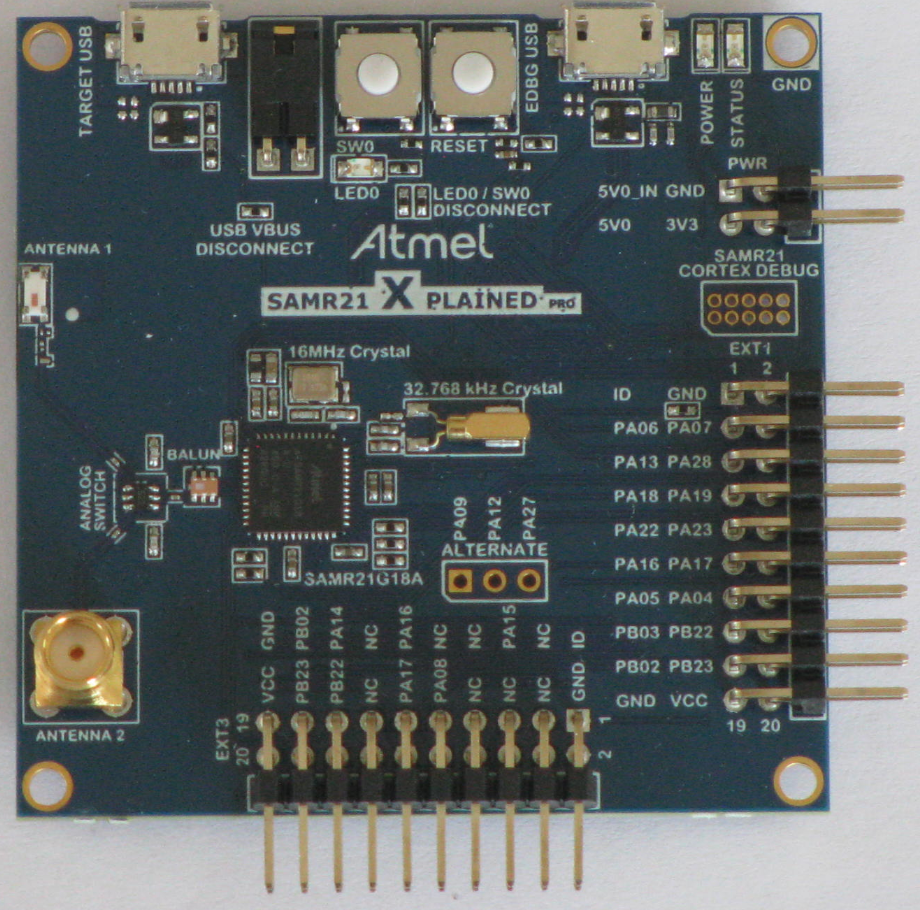
\includegraphics[width=0.6\textwidth]{images/samr21.png}
	\caption{Vorderseite des \board Board}
	\label{img:samr21}
\end{figure}

\subsubsection{Sensoren}
Für die Lauftzeitmessung können verschiedene Sensoren verwendet werden. Folgend ein Vergleich zwischen dem Ultraschallsensor \ultraschall \platz und dem \microphone \platz Sensor. Dieser Vergleich wird durchgeführt, weil beide Sensoren in der Entwicklung zum Einsatz kamen, aber nur einer die nötigen Performance für die Positionsbestimmung leistet.

%als alternative subsubsubsection
\paragraph{Ultraschallsensor}\mbox{}\\
Für die Positionsbestimmung ist der Ultraschallsensor \ultraschall \platz (Abbildung \ref{img:ultraschallsensor}) zum Einsatz gekommen \cite{src_HC_SR04}. Ich habe mich für den \ultraschall \platz Sensor aufgrund seiner weiten Verbreitung im Arduino/ Raspberry Pi Bereich, seiner kompakten Bauweise, der geringen Kosten und der einfachen Ansteuerung entschieden. Ultraschallsensoren werden verwendet, um Distanzen zu einem Gegenstand zu ermittlen. Dabei wird ein Ultraschallsignal ausgesendet und von dem Gegenstand zurück reflektiert und wieder empfangen. Über die Zeitdifferenz zwischen Aussenden und Empfangen des Ultraschallsignals kann die Distanz berechnet werden. Aus der Abbildung \ref{img:ultraschall_prinzip} wird das Prinzip deutlich. Der \ultraschall \platz  hat eine Reichweite von $3\; cm$ bis $4\;m$. Der Vorteil von diesem Ultraschallsensor ist, dass es ohne weitere Sensoren auskommt. Allerdings weißt der Ultraschallsensor einige Nachteile auf, weswegen er von einem leistungsfähigeren Schallmikrofon (\microphone) abgelöst worden ist. Ultraschallsensoren funktionieren nur, wenn sie direkten Sichtkontakt zum Objekt haben. Dies ist nicht immer gegeben. Des weiteren könnnen nur Objekte, die in dem Sendekegel des Ultraschallsensors liegen, detektiert werden. Der Sendekegel für den \ultraschall \platz liegt bei $15^\circ$. Aufgrund dieser Nachteile habe ich mich in der Endanwendung gegen diesen Sensor entschiedenen, denn die Positionsbestimmung wird dadurch stark beeinträchtigt.
\begin{figure}[!ht]
        \centering
        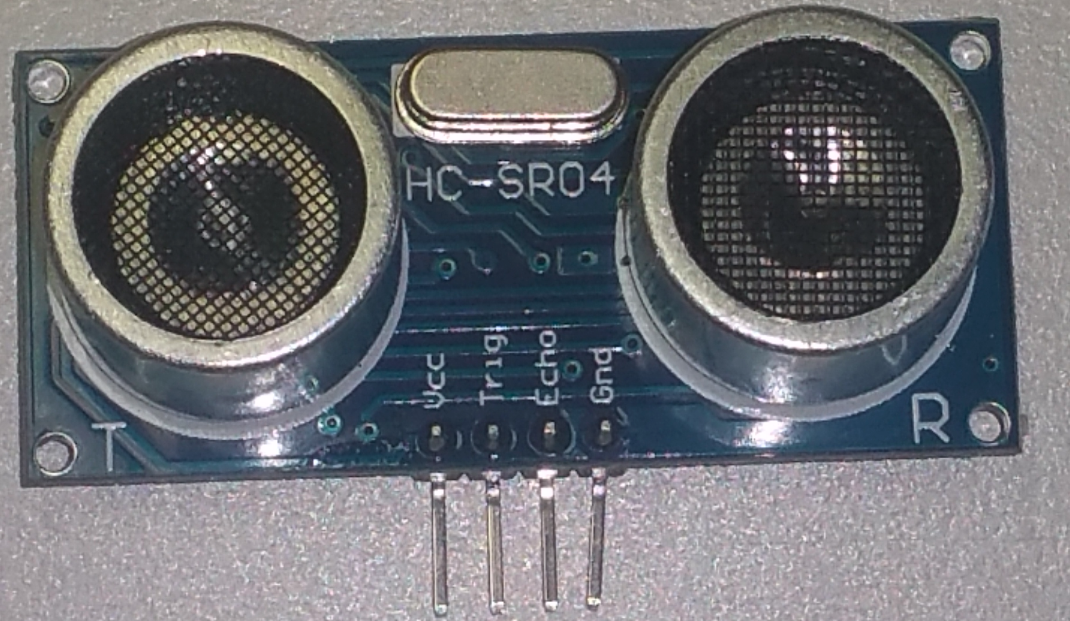
\includegraphics[width=0.6\textwidth]{images/ultraschallsensor.png}
        \caption{Vorderseite des \ultraschall \platz Sensor}
        \label{img:ultraschallsensor}
\end{figure}
\begin{figure}[!ht]
        \centering
        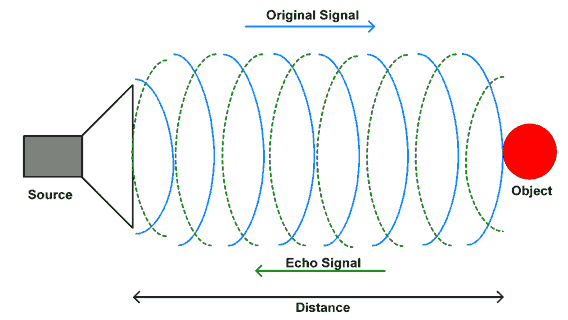
\includegraphics[width=0.6\textwidth]{images/ultraschall_prinzip.png}
        \caption{Funktionsweise von Ultraschallsensoren}
        \label{img:ultraschall_prinzip}
\end{figure}

\paragraph{Sound Detector}\mbox{}\\
Im Verlauf der Umsetzung für die Positionsbestimmung hat sich gezeigt, dass sich der Ultraschallsensor \ultraschall \platz nicht eignet. Abhilfe schafft der \microphone. Abbildung \ref{img:sound} zeigt den \microphone. Der Sensor kann hörbaren Schall detektieren. Darüber hinaus kann die Empfindlichkeit durch das Einlöten eines Widerstandes erhöht oder verringert werden. Der Vorteil gegenüber dem Ultraschallsensor ist, dass der Schall sich kugelförmig ausbreitet. Somit muss der Sensor nicht auf eine Richtung ausgerichtet werden. Allerdings stellen Hindernisse für einen hörbaren Schall ein Problem da. Deswegen sollten keine oder nur wenige Hindernisse auf der Ebene vorhanden sein. Die Reichweite kann über eine Amplitudenveränderung des Tongebers verändert werden. Für die Ansteuerung des \microphone \platz kann der digitale Ausgang \si{GATE} verwendet werden. Sobald ein Signal die eingestellte Schallschwelle überschreitet, wird der \si{GATE} Ausgang des Sound Detectors auf \si{HIGH} gesetzt. Wird die Schallschwelle unterschritten, fällt der \si{GATE} Ausgang zurück auf \si{LOW}. Es gibt noch weitere Ausgänge, allerdings werden diese nicht verwendet \cite{src_SOUND_DETECTOR}. Die Abbildung \ref{img:gate_ausgang} zeigt ein Überschreiten des Schallpegels.

\begin{figure}[H]
        \centering
        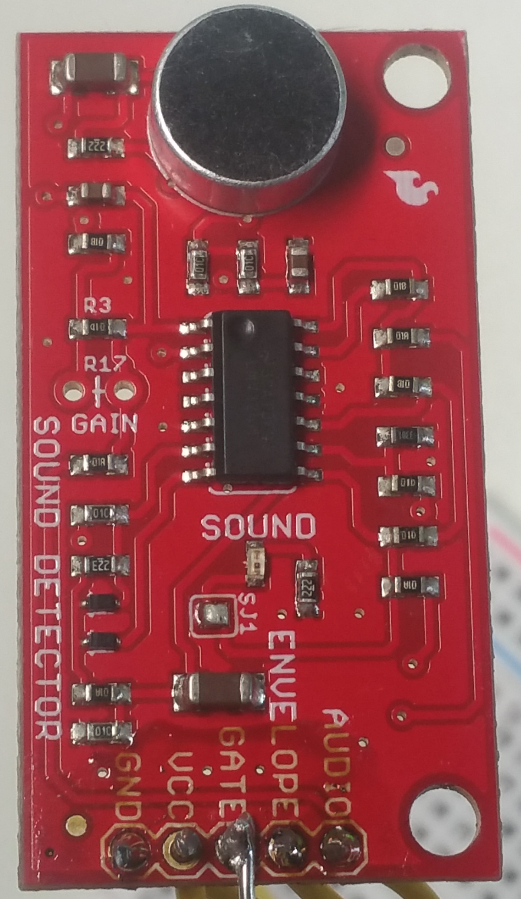
\includegraphics[width=0.4\textwidth]{images/sounddetector.png}
        \caption{Sparkfun Sound Detector}
        \label{img:sound}
\end{figure}
\begin{figure}[H]
        \centering
        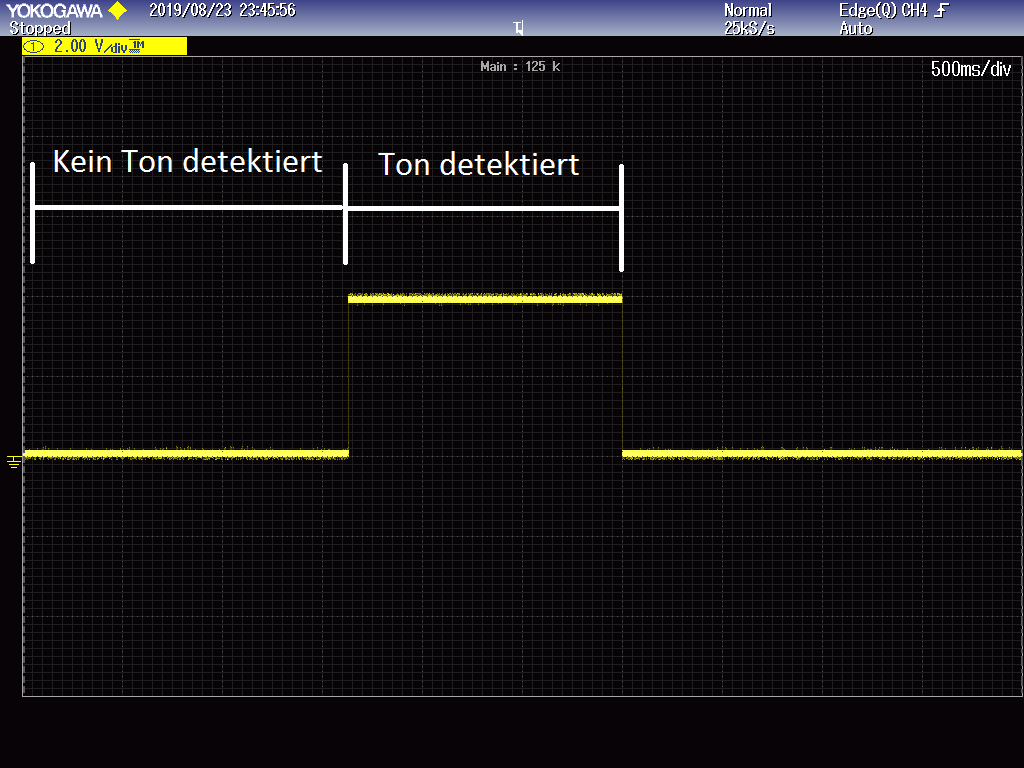
\includegraphics[width=1\textwidth]{images/gate_ausgang.png}
        \caption{Pegelwechsel des \si{GATE}-Ausgang}
        \label{img:gate_ausgang}
\end{figure}

\paragraph{\funkempfaenger}\mbox{}\\
Dieser Funksender sendet auf der \SI{433}{MHz} Frequenz \cite{src_433_FUNKSENDER}. Er ist im Arduino Umfeld weit verbreitet und aufgrund seiner schlichten Ansteuerung einfach zu bedienen. Der Funksender besitzt keine Fehlerkorrektur für verlorene Nachrichten, sowie keine Signalkodierung. Deswegen eignet er sich gut für geringe Bandbreiten. Meine Arbeit verwendet diesen Sensor, um ein Startsignal zu senden. Im laufe der Arbeit hat sich allerdings gezeigt, dass diese Variante nicht fehlerfrei funktioniert. Es folgt ein Foto \ref{img:433_sender_empf} des Sensors.

\begin{figure}[H]
	\hspace*{-2cm}
    \subfigure[Funksender]
    {
    	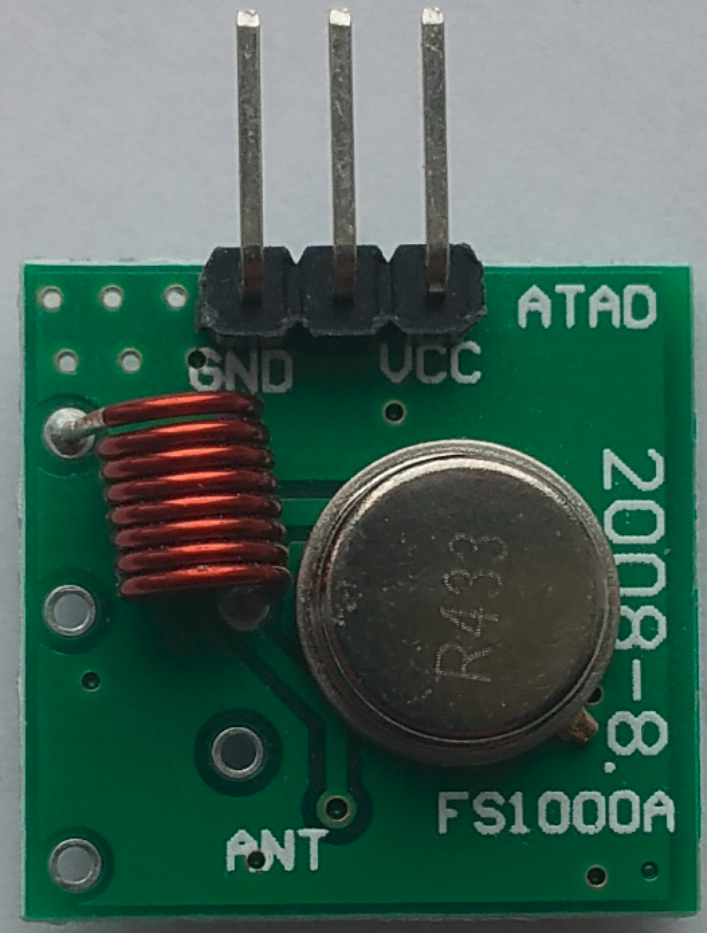
\includegraphics[width=0.5\textwidth]{images/sender.png}
    }	
    \subfigure[Empfänger]
    {
    	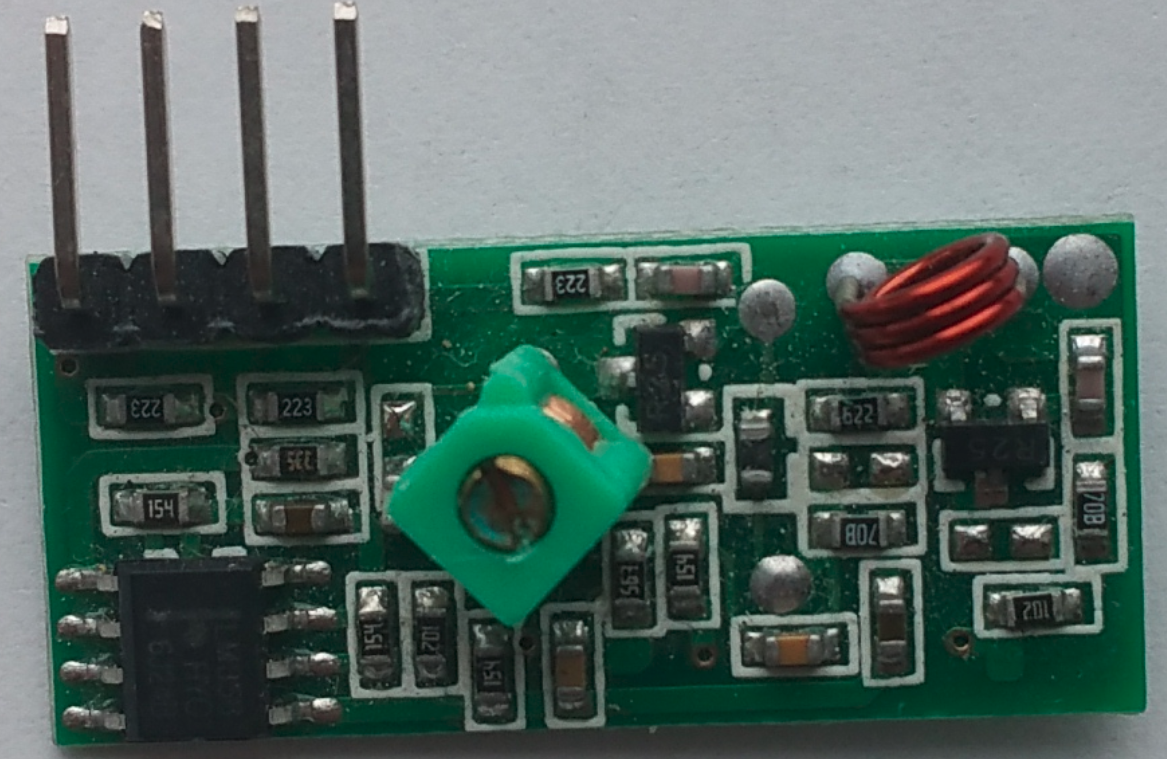
\includegraphics[width=0.7\textwidth]{images/empf.png}
    }
	\caption{\funkempfaenger}
	\label{img:433_sender_empf}
\end{figure}

Es folgt eine Auflistung der Anschlüsse des Funksender von links.
\begin{description}[style=multiline,leftmargin=3cm]
\item [GND] 	Masse
\item [DATA]	Payload
\item [VCC]		Versorgungsspannung
\end{description}
\newpage
Der Empfänger besitzt vier Anschlüsse. Diese sind wie folgt:
\begin{description}[style=multiline,leftmargin=3cm]
\item [GND] 	Masse
\item [DATA]	Payload
\item [DATA]	Payload
\item [VCC]		Versorgungsspannung
\end{description}

Mit einem Pegelwechsel des Funksender bei dem Anschluss \si{DATA} kann eine Nachricht übertragen werden. Der Empfänger gibt die empfangenen Daten über die \si{DATA} Anschlüsse wieder aus. Mithilfe eines Schmitt-Triggers kann dieses Signal geglättet werden.

\paragraph{Lautsprecher}\mbox{}\\
Als Tongeber wird ein handelsüberlicher aktiver Lautsprecher verwendet \cite{src_LAUTSPRECHER}. Im Vergleich zu passiven Lautsprechern, muss die Frequenz nicht selbst erzeugt werden. Mit dem Anlegen der Betriebsspannung wird die Membram in Schwingung versetzt. Die Lautstärke wird über die Betriebsspannung reguliert. Da der Lautsprecher mit \SI{24}{\volt} betrieben wird, benötigt man eine externe Schaltung. Diese besteht aus einem n-dotiertem Mosfet und dem Lautsprecher. Abbildung \ref{img:schaltung} zeigt die Schaltung. Wenn an dem \si{GATE} Eingang des Mosfet eine Spannung von \si{2} - \SI{4}{\volt} anliegt, schaltet der Mosfet durch, und der Lautsprecher wird mit Strom versorgt. 
\begin{figure}[H]
        \centering
	\hspace*{-1.5cm}
        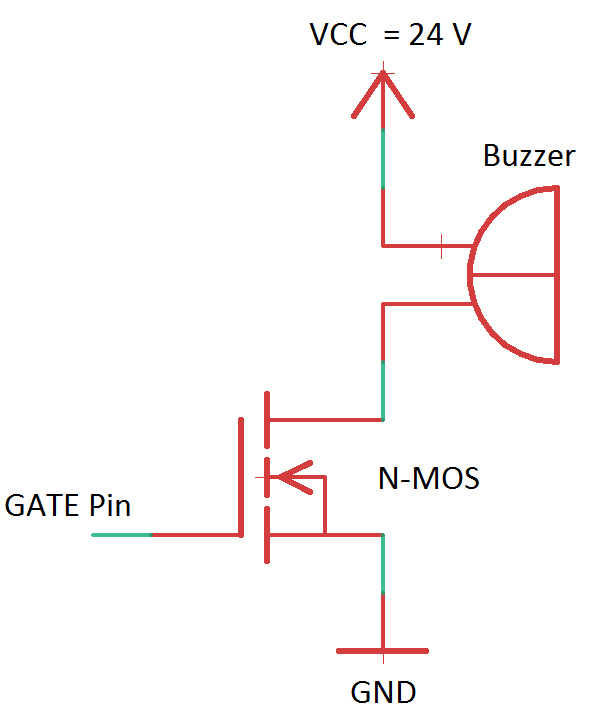
\includegraphics[width=0.65\textwidth]{images/schaltung.png}
        \caption{Ansteuerung des Lautsprechers}
        \label{img:schaltung}
\end{figure}


\subsection{Verwendete Software}
\subsubsection{RIOT OS}
Um das \board \platz in Betrieb zu nehmen, kommt das echtzeitfähige Betriebssystem RIOT zum Einsatz. RIOT steht für: "The friendly Operating System for the Internet of Things" und wurde von der Freien Universität Berlin, der INRIA (Institut national de recherche en informatique et en automatique, Le Chesnay, Frankreich) und der Hochschule für Angewandte Wissenschaften, Hamburg entwickelt. Es entstand aus dem "FeuerWhere" Projekt, bei dem Feuerwehrleute im Einsatz überwacht werden sollten. 2010 kam es zu einer Abspaltung des Projekts - das war die Geburtsstunde von RIOT. RIOT ist ein Betriebssystem für Internet of Things Anwendungen. RIOT hat den Fokus auf drahtlose Sensornetzwerke gelegt. Protokolle wie 6LoWPAN, RPL, UDP und TCP wurden mit der Zeit implementiert. Des weiteren unterstützt RIOT echtes Multithreading. Vergleicht man RIOT mit anderen Embedded Betriebssystemen, erkennt man, dass RIOT, die steigenden Anforderungen an Embedded Betriebssystemen unterstützt. Weiterhin ist RIOT mit dem verwendeten Board \board \platz kompatibel, weswegen es sich perfekt als Betriebssystem für diese Arbeit eignet \cite{src_RIOT}. Die folgende Abbildung \ref{img:vergleich} vergleicht RIOT mit drei anderen Betriebssystemen.

\begin{figure}[H]
        \centering
		\hspace*{-1.5cm}
        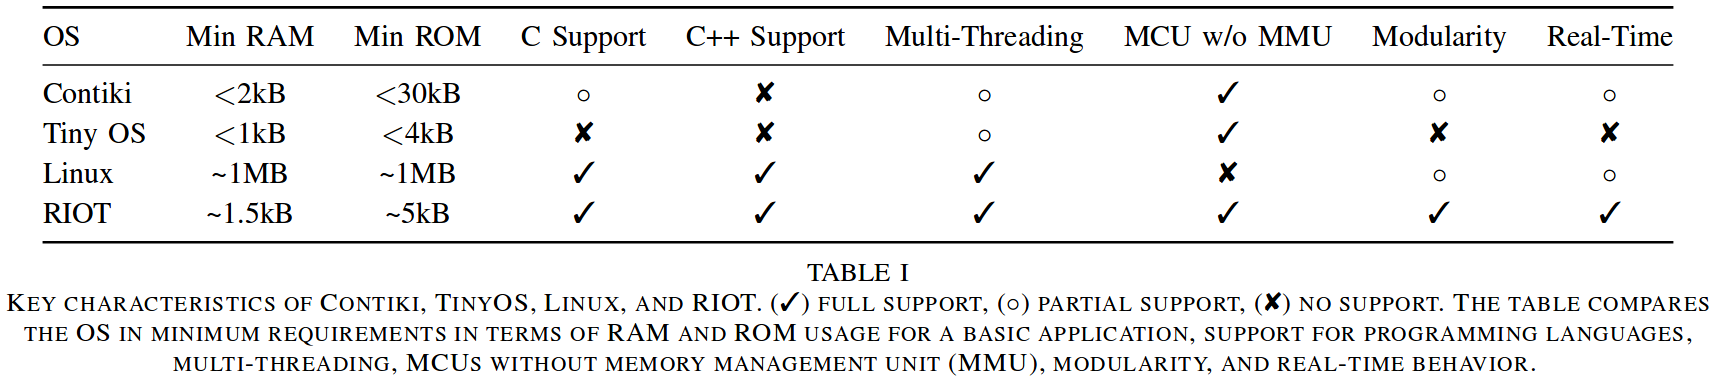
\includegraphics[width=1.2\textwidth]{images/vergleich.png}
        \caption{Vergleich von RIOT mit drei anderen Betriebssystemen}
        \source{https://www.riot-os.org/docs/riot-infocom2013-abstract.pdf}
        \label{img:vergleich}
\end{figure}

\subsection{Time Difference of Arrival - TDOA}
Das TDOA ist ein Verfahren zur Laufzeitmessung, welches den Laufzeitunterschied eines Zeitstempels misst. Damit können Endgeräte über mindestens drei Basisstationen geortet werden. Für die Lauftzeitmessung kann jede Art von Signal verwendet werden \cite{src_TDOA}.

\subsection{User Datagram Protocol - UDP}
UDP ist ein Netzwerkprotokoll, welches im OSI-Modell in Schicht vier zu finden ist. UDP ist 1977 für die Sprachübertragung in Rechnernetzwerken entwickelt worden. Es ist einfach aufgebaut. Es arbeitet verbindungslos, d.h. der Sender bekommt keine automatische Meldung ob das gesendete Paket angekommen ist. Im Gegensatz dazu arbeitet TCP verbindungsorientiert. TCP steht für: Transmission Control Protocol. Es ist wie UDP ein Netzwerkprotokoll zur Datenübertragung.
\\
Des weiteren hat UDP den Vorteil, dass vorher keine Verbindung mit dem Empfänger aufgebaut werden muss. Das ist besonders im IoT- Bereich wichtig, denn dort sind die Systeme meistens batteriebetrieben. Allerdings kann nicht ausgeschlossen werden, dass die Daten unverfälscht beim Empfänger ankommen.
\\
Ein UDP Paket wird unterteilt in ein Headerfeld und ein Datenfeld. Die Größe des Headers sind immer 8 Byte. Es folgt eine Auflistung der Komponenten aus denen das UDP Paket besteht \cite{src_UDP}:

\begin{description}[style=multiline,leftmargin=3cm]
\item [Quellport] 	Port des Quellrechners
\item [Zielport]  	Port des Zielrechners
\item [Länge]		Gibt die Länge des Datensegmentes in Byte an
\item [Prüfsumme]	Ein Wert, der aus dem Datensegment errechnet wird, um Manipulationen zu erkennen
\item [Daten]		Nutzlast
\end{description}

\subsection{Netzwerk-Socket}
Ein Socket ist eine Schnittstelle, die vom Betriebssystem bereitgestellt wird. Ein Socket verbindet einen Kommunikationsendpunkt mit dem Betriebssystem. Über ein Socket kann ein Programm, welches eine Datei ist, auf den Kommunikationsendpunkt zugreifen. Wenn Netzwerkdaten empfangen werden, liegen diese zur Abholung im Socket bereit. Sockets können bidirektional\footnote{Datenübertragung in beide Richtungen} betrieben werden. Sockets sind immer an einen Port gebunden. Dadurch weiß das Betriebssystem, welche Pakete zu welchem Socket gehören. Im Gegenzug gibt es noch die RAW-Sockets. Diese erlauben den Zugriff auf das ganze Paket. Dort werden keine Daten vorher aus dem Paket gefiltert \cite{src_SOCKET}.

\subsection{Indoor/Outdoor Positionsbestimmung}
Indoor-Positionsbestimmungssysteme sind nicht so weit verbreitet wie Outdoor-Systeme. Für Outdoor-positionsbestimmungen wird häufig das globale Navigationssatellitensystem GPS (Global Positioning System) verwendet. Es kann aber auch der Mobilfunk verwendet werden. Für die Positionsbestimmung im Indoorbereich existieren mehrere Verfahren. Dazu zählen Messungen des Einfallswinkels, Signalstärkemessungen oder Laufzeitmessungen. Da wir bereits entschieden haben, dass wir Schall für die Positionsbestimmung nehmen, verwenden wir das Verfahren der Laufzeitmessung. Dabei wird die Zeitdifferenz zwischen Sende- und Empfangszeit ermittelt, sodass man die Signallaufzeit erhält \cite{src_INDOOR_OUTDOOR_SYSTEME}. Zusammen mit der Ausbreitungsgeschwindigkeit von Schall ($343,2 \frac{m}{s}$ bei \SI{20}{\degreeCelsius}) kann die Distanz über die folgende Formel \ref{eq:formel_laufzeitmessung} berechnet werden:
\begin{equation}
   Distanz \;[m] = (Empfangszeit - Sendezeit)\;[sec]\quad \cdot Ausbreitungsgeschwindigkeit \;[m/sec]
   \label{eq:formel_laufzeitmessung}
\end{equation}

\subsection{Zeitsynchronisation}
Für eine Laufzeitmessung ist es wichtig, dass Sender und Empfänger die gleiche Uhrzeit haben. Damit eine hohe Genauigkeit bei der Laufzeitmessung erreicht wird kann, muss der Zielknoten (Master) wissen, zu welchem Zeitpunkt der Accesspoint (Slave) den Schall, aussendet. Ist dies nicht gewährleistet, muss der Master raten. Damit nicht geraten werden muss, ist es notwendig, dass beide Knoten die gleiche Zeitbasis haben. Für dieses Problem wird eine Zeitsynchronisation für drahtlose Netzwerke verwendet, das Precision Time Protocol (PTP). PTP ist für drahlose Sensornetzwerke entwickelt worden - es gibt hierbei keine Hierachien wie beim Network Time Protocol. Der Vorteil liegt darin, dass PTP nicht mit jeder Hierachie Genauigkeit verliert wie NTP. Es spezialisiert sich auf kleine Netzwerke ohne Hiearchien. Eine Genauigkeit im Nanosekundenbereich kann erreicht werden, wenn die aktuelle Systemzeit kurz vor dem Absenden des Pakets hinzugefügt wird. Desto geringer die Verzögerung zwischen dem Funktionsaufruf $getSystemTime()$ und dem Absenden des Pakets, desto genauer wird die Zeitsynchronisation. Die folgende Abbildung \ref{img:ptp} zeigt, welchen Nachrichtenaustauch für die Zeitsynchronisation nötig ist \cite{src_PTP}. Der Master ist der Sender und der Slave ist der Empfänger.

\begin{figure}[H]
        \centering
%		\hspace*{-1.5cm}
        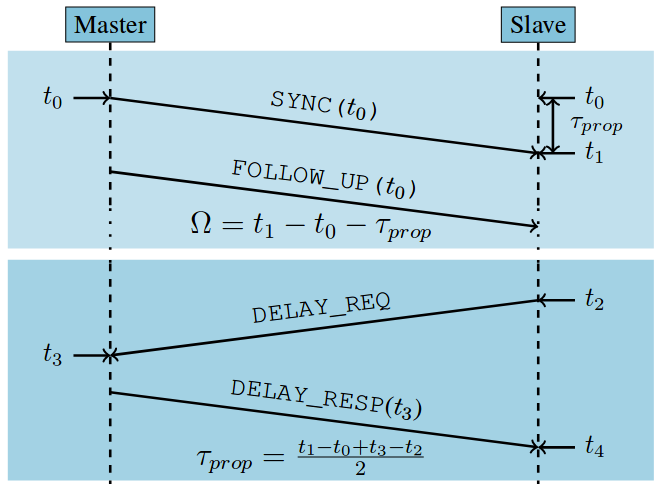
\includegraphics[width=0.9\textwidth]{images/ptp.png}
        \caption{Nachrichtenaustausch in PTP}
        \source{https://www.ibr.cs.tu-bs.de/oa/vonzengen\_ICIT2017.pdf}
        \label{img:ptp}
\end{figure}

Zuerst sendet der Master eine \si{SYNC} Nachricht mit seinem Zeitstempel $t_{0}$ an den Slave. Aufgrund der Verarbeitungszeit, der Laufzeitverzögerung und der Zugriffszeit, ist der Zeitstempel $t_{0}$ für den Slave nicht präzise. Mit einer \si{FOLLOW\_UP} Nachricht werden diese Probleme gemildert. Dabei enthält die \si{FOLLOW\_UP} Nachricht den Zeitstempel $t_{0}$. Nachdem beide Nachrichten beim Slave angekommen sind, antwortet der Slave mit einer \si{DELAY\_REQ} Nachricht - ohne Inhalt. Der Master sendet darauf hin ein \si{DELAY\_RESP} mit dem Zeitstempel $t_{3}$. Nun kann mit den folgenden zwei Formeln \ref{eq:formel_ptp} die Zeitdifferenz berechnet werden. Dabei entspricht $\tau_{prop}$ den Zeitunterschied zwischen beiden Systemen und Omega ($\Omega$) ist der Offset zwischen Master und Slave.

\begin{equation}\label{eq:formel_ptp}
\begin{split}
\tau_{prop} = \frac{t_{1} - t_{0} + t_{3} - t_{2}}{2}
\\
\Omega = t_{1} - t_{0} - \tau_{prop}
\end{split}
\end{equation}


\subsection{Mathematischer Hintergrund - Positionsbestimmung}

Damit auf einer Ebene die Position bestimmt werden kann, muss der Master von mindestens drei Slaves die Distanz messen. Da sich der Schall auf einer Ebene kreisförmig ausbreitet, vereinfacht sich das Problem auf den Schnittpunkt von drei Kreisen (Abbildung \ref{img:positionsbestimmung}). Des weiteren müssen die Koordinaten der Slaves bekannt sein.
\begin{figure}[H]
        \centering
%		\hspace*{-1.5cm}
        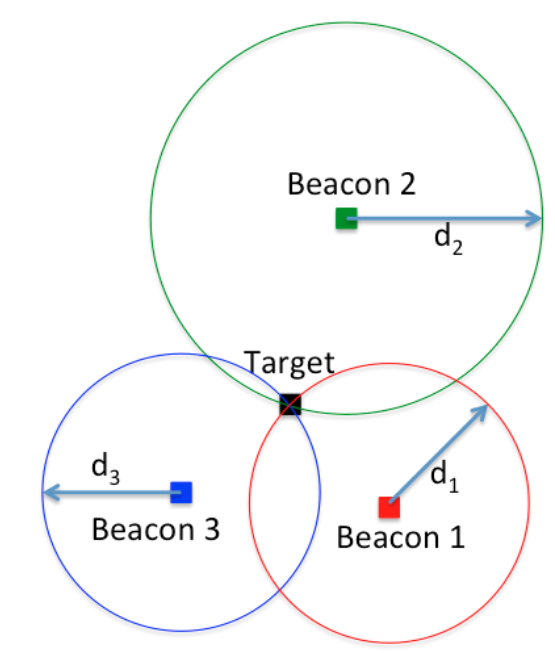
\includegraphics[width=0.5\textwidth]{images/positionsbestimmung.png}
        \caption{Prinzip der Positionsbestimmung}
		\source{https://sites.tufts.edu/eeseniordesignhandbook/files/2017/05/FireBrick\_OKeefe\_F1.pdf}
        \label{img:positionsbestimmung}
\end{figure}
Aufgrund von Schwankungen kann es sein, dass es keinen gemeinsamen Schnittpunkt der drei Kreise gibt, wie Abbildung \ref{img:positionsbestimmung} vermittelt. Deswegen wird ein Bereich angegeben, wo sich der Master befinden muss. Je größer die Schwankungen bei der Distanzmessung sind, desto größer ist der Zielbereich \cite{src_MATH_TDOA}. Abbildung \ref{img:schwankungen} verdeutlicht das Problem. Dort befindet sich der Master zwischen den folgenden Punkten:

\begin{equation}
\begin{split}
A: \; (2,7671\;|\;3,3700) \\
B: \; (3,1775\;|\;2,5081) \\
C: \; (2,2727\;|\;1,4454)
\end{split}
\end{equation}


\begin{figure}[H]
        \centering
%		\hspace*{-2.7cm}
        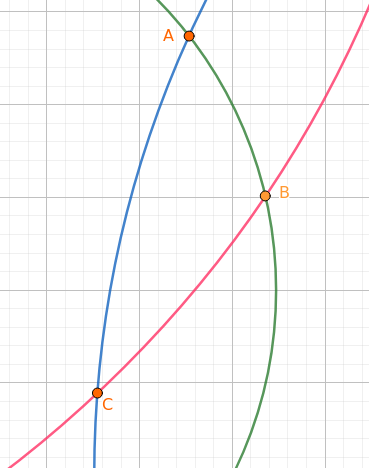
\includegraphics[width=0.7\textwidth]{images/positionsbestimmung_flaeche.png}
        \caption{Bereich indem sich der Zielknoten befinden muss}
        \label{img:schwankungen}
\end{figure}

Die Normalform für eine Kreisgleichung mit Mittelpunkt $(x_{0}|y_{0})$ und Radius $r$ lautet:
\begin{equation}
(x-x_{0})^{2}+(y-y_{0})^{2} = r^{2}
\end{equation}

Mit Hilfe der drei Kreise (A, B, C) (Abbildung \ref{img:positionsbestimmung}) kann nun der Schnittpunkt berechnet werden. - siehe folgendes Gleichungssystem \ref{eq:gleichungssystem}. Dabei entsprechen $x_{A}$, $y_{A}$ den Mittelpunkt von Kreis $A$ mit Radius $r_{A}$. Diese Notation wird auch auf Kreis $B$ und $C$ angewendet.

\begin{equation} \label{eq:gleichungssystem}
\begin{split}
\RM{1} \quad (x-x_{A})^{2}+(y-y_{A})^{2} &= r_{A}^{2} \\
\RM{2} \quad (x-x_{B})^{2}+(y-y_{B})^{2} &= r_{B}^{2} \\
\RM{3} \quad (x-x_{C})^{2}+(y-y_{C})^{2} &= r_{C}^{2}
\end{split}
\end{equation}

Um den Schnittpunkt zwischen allen drei Kreisen zu erhalten, muss das Gleichungssystem \ref{eq:gleichungssystem} nach $x$ und $y$ aufgelöst werden. Aufgrund von Schwankungen ist dies nicht immer möglich. Punkt $1$ berechnet sich durch das Auflösen nach $x$ von $\RM{1}$ und $\RM{2}$ . Für Punkt $2$ werden die Gleichungen $\RM{1}$ und $\RM{3}$ verwendet, für den dritten Punkt $\RM{2}$ und $\RM{3}$. Die Herleitung ist im Anhang aufgeführt. 


\newpage
\section{Entwurf}
Dieses Kapitel befasst sich mit der Sruktur der Implementierung. Damit wird die Herangehensweise beschrieben und es wird erläutert, wieso bestimmte Entscheidungen getroffen worden sind.

\subsection{Hardware}
Um die Hardwarekosten bei einer Skalierung für die Positionsbestimmung niedrig zu halten, wurde der \microphone \platz auf dem Master-Knoten verbaut und dementsprechend die Lautsprecher auf dem Slave-Knoten. Diese Variante hat allerdings den Nachteil, dass nur ein Slave abgefragt werden kann. Somit braucht es bei drei Slaves mindestens drei Schallmessungen, gegenüber einer Messung. Die verwendetete Variante hat jedoch den Vorteil, dass der Master entscheidet, mit welchem Slave eine Messung vorgenommen wird. Weiterhin ist der Softwareaufwand für eine Wiederholung der Messung aufgrund von Fehlern geringer.

\subsection{Struktur}
Zuerst wird der \microphone \platz dahingehend untersucht, ob er überhaupt schnell genug für die Positionsbestimmung ist. Danach wird ein Versuchsaufbau nach dem folgenden Blockschaltbild \ref{img:kommunikation_module}, eingerichtet. Das Blockschaltbild teilt den Versuchsaufbau in verschiedene Module auf -- damit lassen sich Abweichungen besser zuordnen.

\begin{figure}[H]
	\centering
	\hspace*{-2.6cm}
	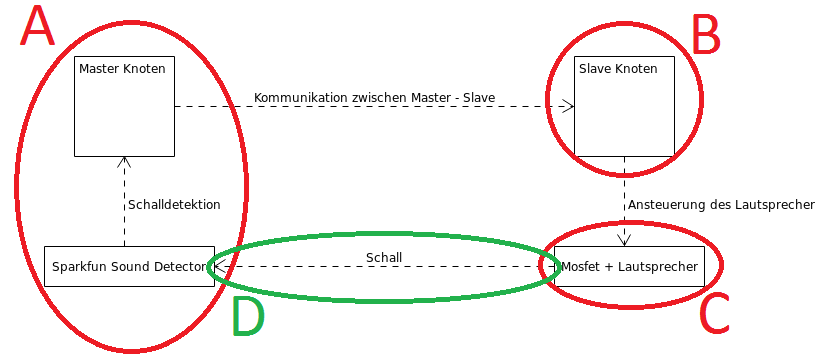
\includegraphics[width=1.3\textwidth]{images/Kommunikation_Module.png}
	\caption{Versuchsaufbau, unterteilt in Module}
	\label{img:kommunikation_module}
\end{figure}

%newpage einfügen

Nachdem die einzelnen Module getestet worden sind, wird der Aufruf der RIOT Funktion $getSystemTime()$ geprüft. Die Prüfung dieser Funktion ist wichtig, weil sie die aktuelle Systemzeit ausliest. Sobald der Ton das Mikrofon passiert, wird diese Funktion aufgerufen. Im Rahmen des Funktionsaufrufes entsteht eine zeitliche Abweichung mit einer hohen Relevanz, da mehrere CPU-Zyklen benötigt werden, bevor die Systemzeit in der Variable gespeichert wird. Anschließend wird die Zeitsynchronisation überprüft. Danach folgt ein Versuch, bei dem anstatt der Funkkommunikation vom \board, das \funkempfaenger \platz Modul verwendet wird. Die verwendete Software für die einzelnen Module ist auf dem mitgelieferten USB-Stick gespeichert. Bei den einzelnen Modulen ist der \si{GATE}-Pin bei dem Master an dem Pin \si{PB23} angeschlossen. Für den Slave wird immer Pin \si{PA18} verwendet. Abbildung \ref{img:verdrahtungsplan_master} und \ref{img:verdrahtungsplan_slave} zeigen die Verdrahtungen.

\begin{figure}[H]
	\centering
	\hspace*{-2cm}
	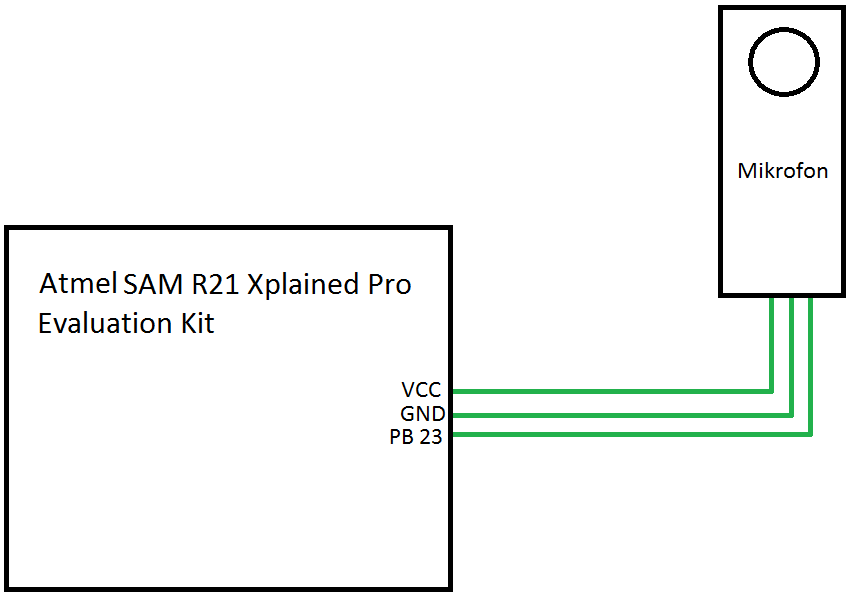
\includegraphics[width=0.6\textwidth]{images/schaltplan_master.png}
	\caption{Verdrahtungsplan Master}
	\label{img:verdrahtungsplan_master}
\end{figure}

\begin{figure}[H]
	\centering
	\hspace*{-2cm}
	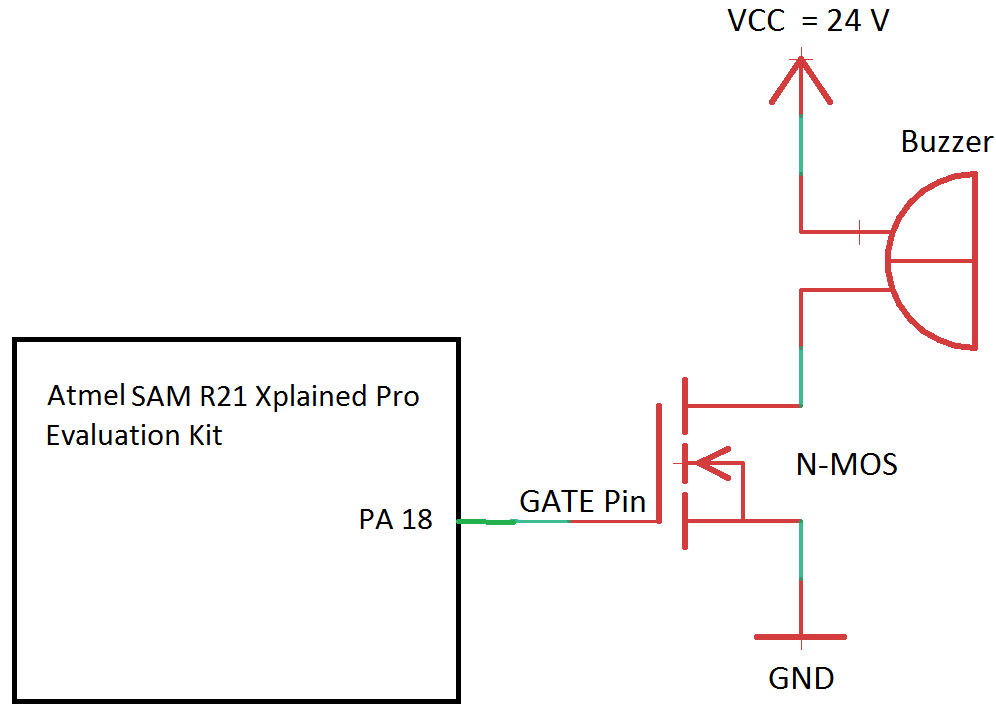
\includegraphics[width=0.6\textwidth]{images/schaltplan_slave.png}
	\caption{Verdrahtungsplan Slave}
	\label{img:verdrahtungsplan_slave}
\end{figure}





\newpage
\section{Implementierung}
Dieses Kapitel widmet sich der der konkreten Implementierung.

\subsection{\microphone}
Bevor eine Messung mit dem Board durchgeführt wird, ist zuerst ein Plausibilitätscheck durchgeführt worden. Dabei überprüft man, ob die beiden \microphone \platz Mikrofone korrekte Ergebnisse liefern. Der Aufbau ist durch das folgende Blockschaltbild \ref{img:blockschaltbild_plausibilitaetscheck} abgebildet. Abbildung \ref{img:picture_plausibilitaetscheck} zeigt den Aufbau im Laborraum.

\begin{figure}[H]
        \centering
        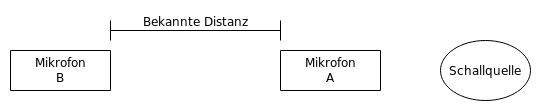
\includegraphics[width=0.9\textwidth]{images/plausibilitaetscheck.png}
        \caption{Versuchsaufbau als Blockschaltbild}
        \label{img:blockschaltbild_plausibilitaetscheck}
\end{figure}

\begin{figure}[H]
        \centering
        \hspace*{-1.9cm}
        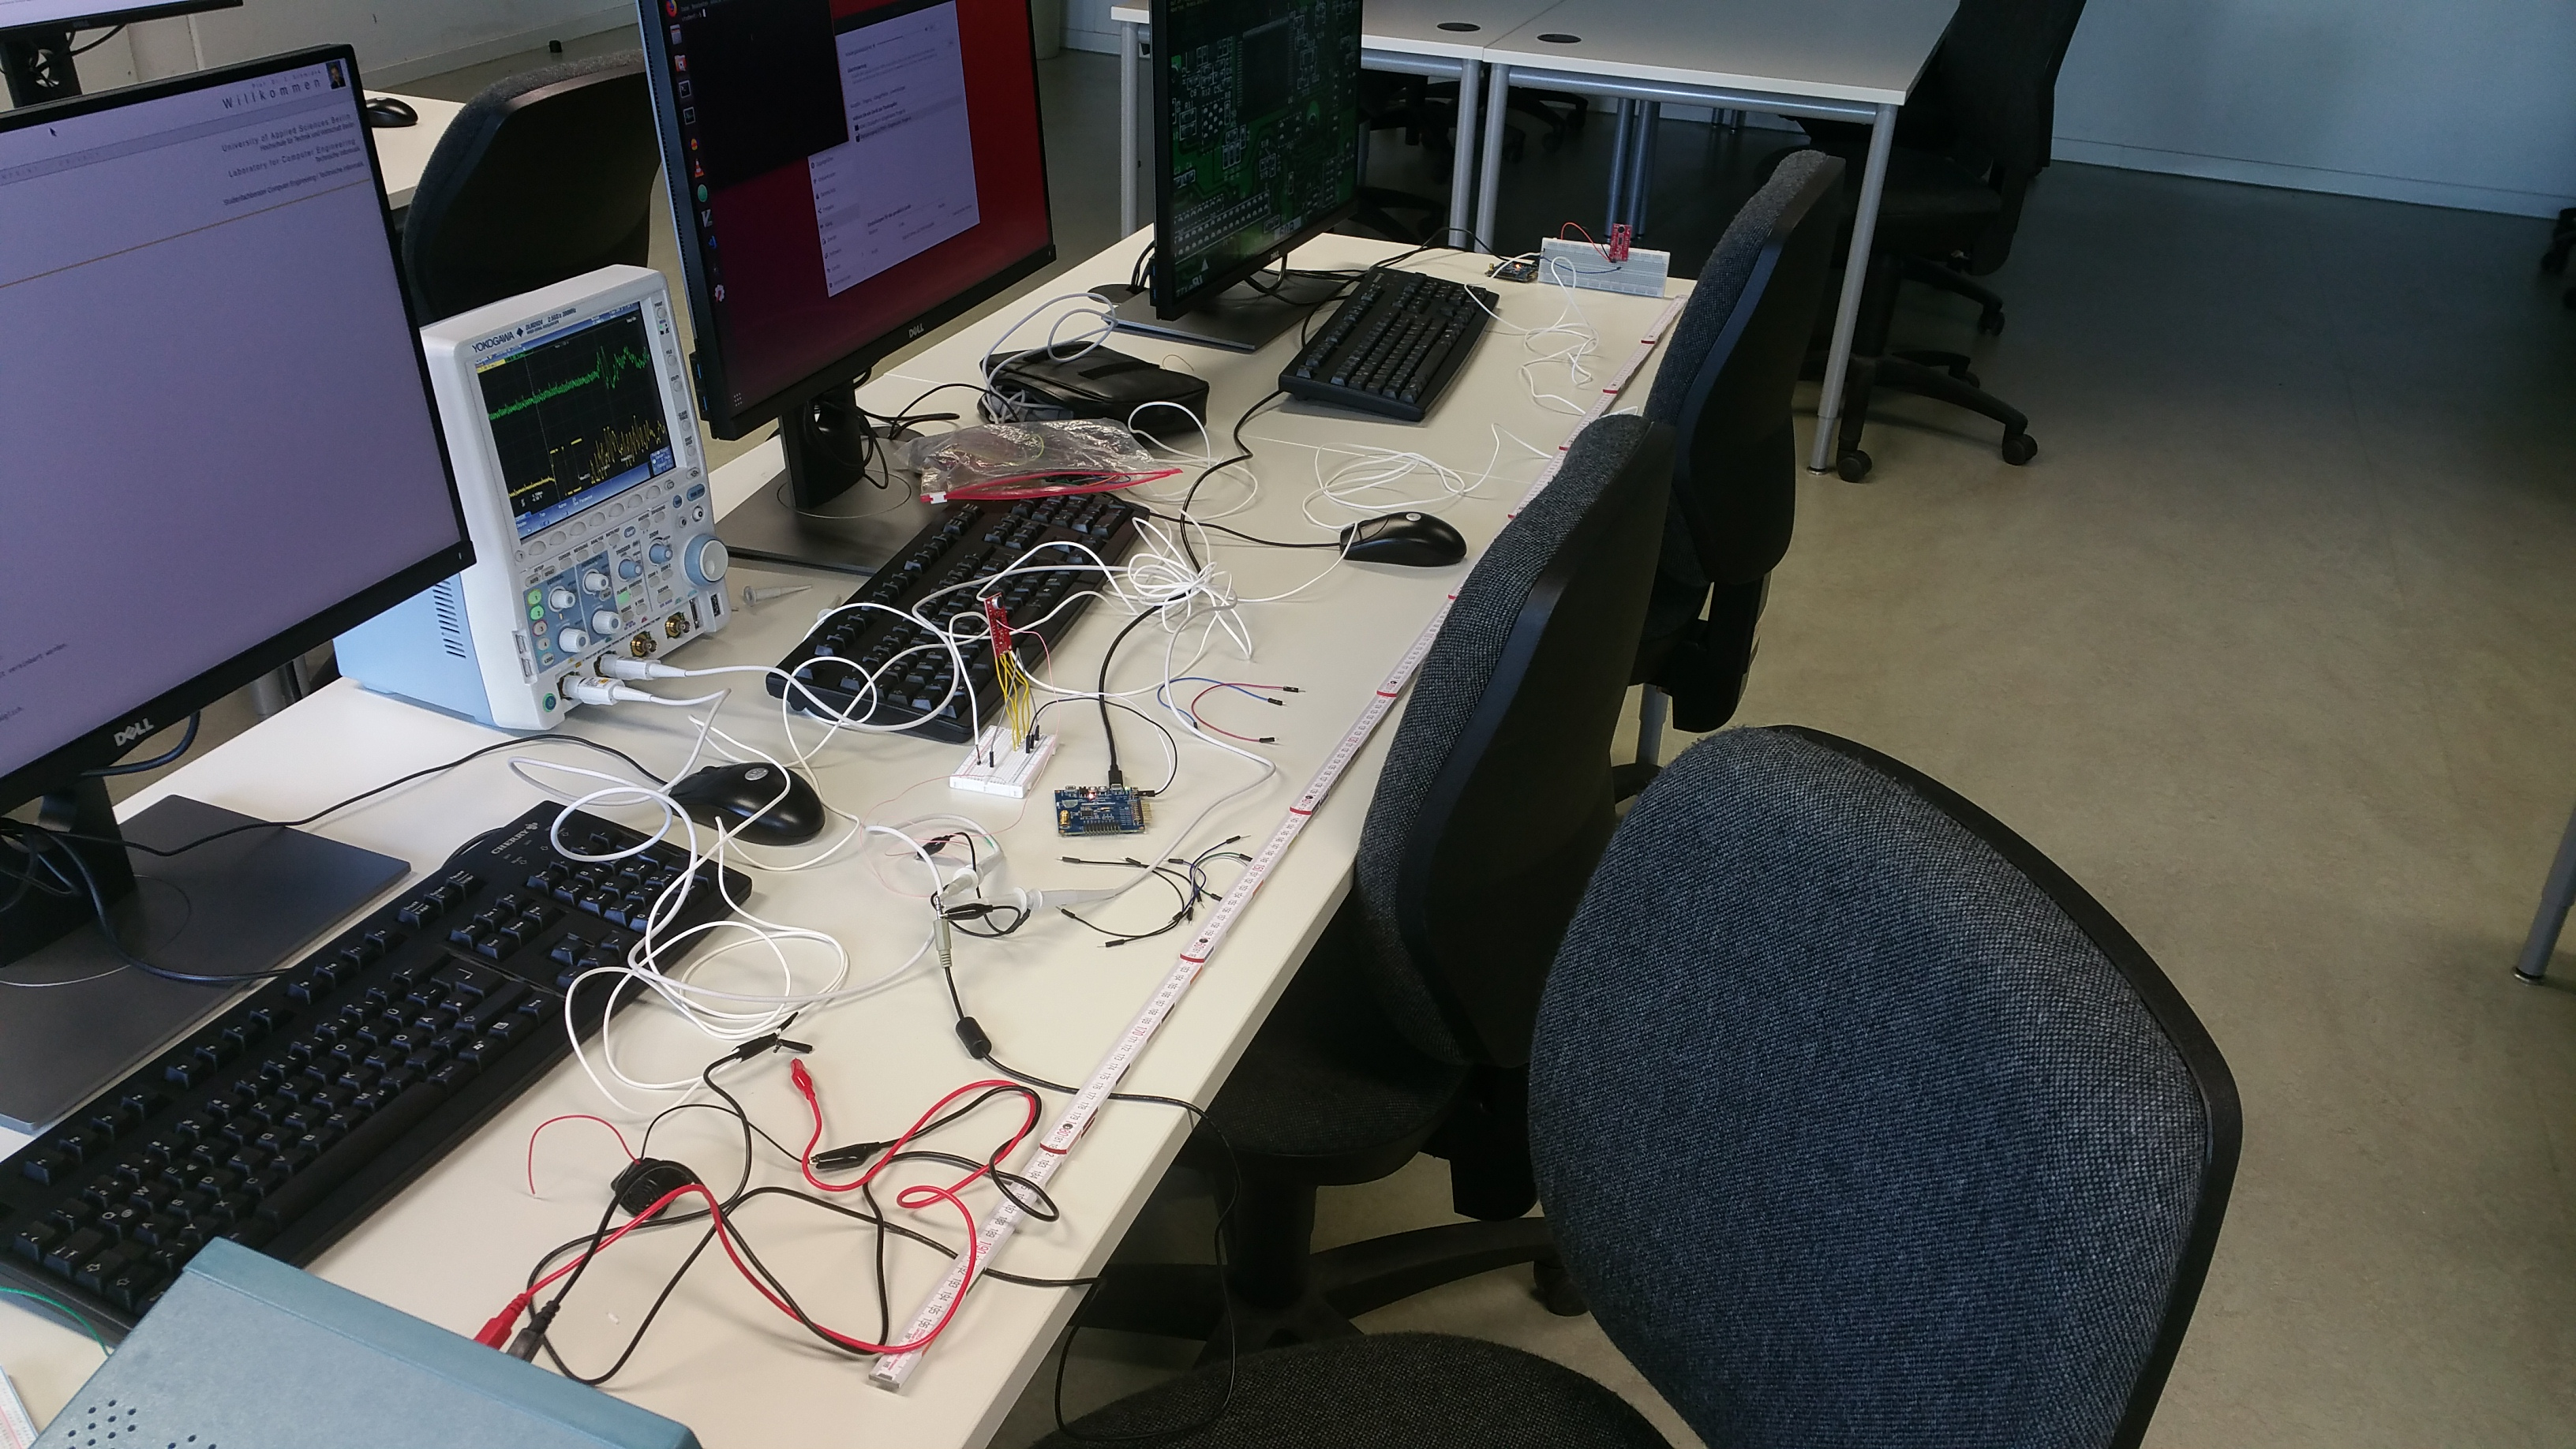
\includegraphics[width=1.2\textwidth]{images/plausibilitaetscheck_sparkfun_foto.jpg}
        \caption{Versuchsaufbau}
        \label{img:picture_plausibilitaetscheck}
\end{figure}

Die beiden Mikrofone sind an einem Oszilloskop angeschlossen. Es werden die \si{AUDIO}- und \si{GATE}-Ausgänge untersucht. Wenn die Schallquelle einen Ton aussendet (durch Klatschen oder ähnliches), passiert er zuerst das Mikrofon A und dann mit einer Verzögerung Mikrofon B. Mithilfe des bekannten Abstandes der beiden Mikrofone wird untersucht, ob das Ergebnis auf dem Oszilloskop mit dem Abstand der Mikrofone übereinstimmt. In Abbildung \ref{img:plausibilitaetscheck_oszi} sind vier verschiedene Signale abgebildet. Dabei entspricht Signal \textit{gelb} dem \si{GATE}-Ausgang von Mikrofon A und \textit{grün} dem \si{AUDIO}-Ausgang. Signal \textit{violett} und \textit{blau} entsprechen dem \si{GATE}- und \si{AUDIO}-Ausgang von dem zweiten Mikrofon.

\begin{figure}[H]
        \centering
        \hspace*{-1.9cm}
        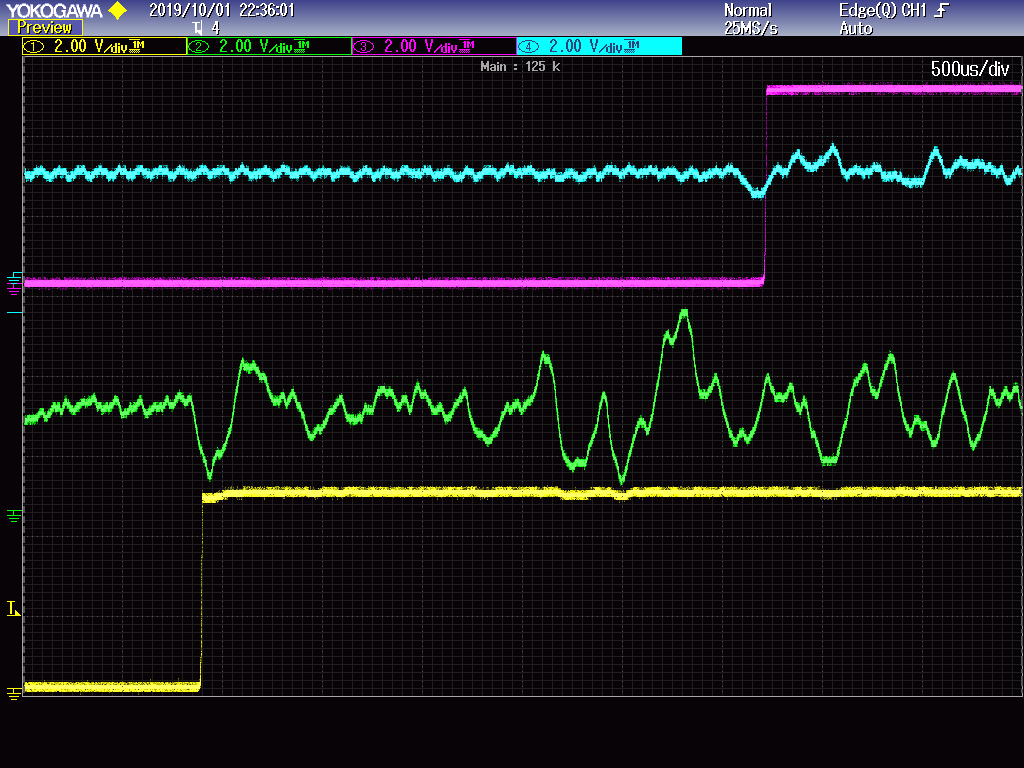
\includegraphics[width=1.2\textwidth]{images/plausibilitaetscheck_oszi.png}
        \caption{Verzögerung der Schallausbreitung}
        \label{img:plausibilitaetscheck_oszi}
\end{figure}

Es ist deutlich erkennbar, dass eine Verzögerung vorhanden ist. Die beiden \si{GATE}-Ausgänge liegen ungefähr \SI{2863}{\micro \second} auseinander. Mit einer Ausbreitungsgeschwindigkeit von \SI{0,034}{\centi\metre\per\micro\second} entspricht das ungefähr \SI{97,342}{\centi\metre}. Der gemessene Abstand ist \SI{100}{\centi\metre}. Diese Auswertung zeigt, dass die Verzögerung nur minimal von dem gemessenen Abstand abweicht. Es folgen weitere Messungen, bei dem anstatt eines Klatschen der verwendetete Tongeber verwendet wird. Dabei sitzt der Lautsprecher direkt neben einem der beiden Mikrofone. Das zweite Mikrofon sitzt \SI{1}{\metre}, \SI{2}{\metre} und \SI{3}{\metre} entfernt. Es folgen drei Tabellen (\ref{tab:plausibilitaetscheck_1m} - \ref{tab:plausibilitaetscheck_3m}) mit den Messwerten (Arithmetisches Mittel).


\begin{table}[H]
\centering
\caption{Messwerte bei \SI{1}{m} Entfernung}
\label{tab:plausibilitaetscheck_1m}
\begin{tabular}{|c|c|c|c|}
\hline
\multicolumn{4}{|c|}{\textbf{\SI{1}{m} Entfernung}}	\\ \hline
\textbf{Messwert von Mikrofon 1 [\si{\mu s}]} & \textbf{Messwert von Mikrofon 2 [\si{\mu s}]} & \textbf{Differenz [\si{\mu s}]} & \textbf{Distanz [\si{\centi\m}]}\\ \hline
\si{595,00}	 & 	\si{4345,00}	 & 	\si{3750,00}	 & 	\si{127,50}	 \\ \hline
\si{603,00}	 & 	\si{4340,00}	 & 	\si{3737,00}	 & 	\si{125,05}	 \\ \hline
\si{461,00}	 & 	\si{4440,00}	 & 	\si{3979,00}	 & 	\si{135,28}	 \\ \hline
\si{608,00}	 & 	\si{4560,00}	 & 	\si{3952,00}	 & 	\si{134,36}	 \\ \hline
\si{641,00}	 & 	\si{4670,00}	 & 	\si{4029,00}	 & 	\si{136,98}	 \\ \hline
\si{443,00}	 & 	\si{4400,00}	 & 	\si{3957,00}	 & 	\si{134,53}	 \\ \hline
\si{450,00}	 & 	\si{4415,00}	 & 	\si{3965,00}	 & 	\si{134,81}	 \\ \hline
\si{634,00}	 & 	\si{4335,00}	 & 	\si{3701,00}	 & 	\si{125,83}	 \\ \hline
\si{638,00}	 & 	\si{4425,00}	 & 	\si{3787,00}	 & 	\si{128,75}	 \\ \hline
\si{640,00}	 & 	\si{4850,00}	 & 	\si{4210,00}	 & 	\si{143,14}	 \\ \hline
\multicolumn{4}{|c|}{\textbf{Durchschnitt}}                    			\\ \hline
\si{571,30}	 & 	\si{4036,50}	 & 	\si{3511,00}	 & 	\si{132,62}	 \\ \hline
\end{tabular}
\end{table}

\begin{table}[H]
\centering
\caption{Messwerte bei \SI{2}{m} Entfernung}
\label{tab:plausibilitaetscheck_2m}
\begin{tabular}{|c|c|c|c|}
\hline
\multicolumn{4}{|c|}{\textbf{\SI{2}{m} Entfernung}} \\ \hline
\textbf{Messwert von Mikrofon 1 [\si{\mu s}]} & \textbf{Messwert von Mikrofon 2 [\si{\mu s}]} & \textbf{Differenz [\si{\mu s}]} & \textbf{Distanz [\si{\centi\m}]}\\ \hline
\si{476,00}	 & 	\si{20150,00}	 & 	\si{19674,00}	 & 	\si{668,91}	 \\ \hline
\si{458,00}	 & 	\si{37900,00}	 & 	\si{37442,00}	 & 	\si{1273,02}	 \\ \hline
\si{471,00}	 & 	\si{36150,00}	 & 	\si{35679,00}	 & 	\si{1213,08}	 \\ \hline
\si{681,00}	 & 	\si{38750,00}	 & 	\si{38079,00}	 & 	\si{1294,68}	 \\ \hline
\si{452,00}	 & 	\si{38150,00}	 & 	\si{37698,00}	 & 	\si{1281,73}	 \\ \hline
\si{466,00}	 & 	\si{34150,00}	 & 	\si{33684,00}	 & 	\si{1145,25}	 \\ \hline
\si{675,00}	 & 	\si{38750,00}	 & 	\si{38075,00}	 & 	\si{1294,55}	 \\ \hline
\si{450,00}	 & 	\si{33550,00}	 & 	\si{33100,00}	 & 	\si{1125,40}	 \\ \hline
\si{447,00}	 & 	\si{32600,00}	 & 	\si{32153,00}	 & 	\si{1093,20}	 \\ \hline
\si{460,00}	 & 	\si{35800,00}	 & 	\si{35340,00}	 & 	\si{1201,56}	 \\ \hline
\multicolumn{4}{|c|}{\textbf{Durchschnitt}}                   	 		\\ \hline
\si{503,60}	 & 	\si{34595,00}	 & 	\si{34072,40}	 & 	\si{1159,13}	 \\ \hline
\end{tabular}
\end{table}

\begin{table}[H]
\centering
\caption{Messwerte bei \SI{3}{m} Entfernung}
\label{tab:plausibilitaetscheck_3m}
\begin{tabular}{|c|c|c|c|}
\hline
\multicolumn{4}{|c|}{\textbf{\SI{3}{m} Entfernung}} \\ \hline
\textbf{Messwert von Mikrofon 1 [\si{\mu s}]} & \textbf{Messwert von Mikrofon 2 [\si{\mu s}]} & \textbf{Differenz [\si{\mu s}]} & \textbf{Distanz [\si{\centi\m}]}\\ \hline
\si{454,00}	 & 	\si{33450,00}	 & 	\si{32996,00}	 & 	\si{1121,86}	 \\ \hline
\si{428,50}	 & 	\si{35800,00}	 & 	\si{35371,50}	 & 	\si{1202,63}	 \\ \hline
\si{474,00}	 & 	\si{37650,00}	 & 	\si{37176,00}	 & 	\si{1263,98}	 \\ \hline
\si{429,00}	 & 	\si{33500,00}	 & 	\si{33071,00}	 & 	\si{1124,41}	 \\ \hline
\si{437,50}	 & 	\si{37700,00}	 & 	\si{37262,50}	 & 	\si{1266,92}	 \\ \hline
\si{439,50}	 & 	\si{35550,00}	 & 	\si{35110,50}	 & 	\si{1193,75}	 \\ \hline
\si{435,50}	 & 	\si{25200,00}	 & 	\si{24764,50}	 & 	\si{841,99}	 \\ \hline
\si{437,50}	 & 	\si{23800,00}	 & 	\si{23362,50}	 & 	\si{794,32}	 \\ \hline
\si{430,00}	 & 	\si{24950,00}	 & 	\si{24520,00}	 & 	\si{833,68}	 \\ \hline
\si{427,50}	 & 	\si{25800,00}	 & 	\si{25372,50}	 & 	\si{862,66}	 \\ \hline
\multicolumn{4}{|c|}{\textbf{Durchschnitt}}                 			\\ \hline
\si{439,30}	 & 	\si{31340,00}	 & 	\si{30900,70}	 & 	\si{1050,62}	 \\ \hline
\end{tabular}
\end{table}


Aus den obigen Tabellen ist zu erkennen, dass Mikrofon \si{1} mindestens \SI{439,30}{\mu\s} braucht, um den Ton wahrzunehmen. Allerdings steht das Mikrofon \si{1} direkt neben dem Tongeber. Durch Latenzen beim Mikrofon ist dieser Messwert nicht null. Allerdings nimmt die Latenz mit der Entfernung ab, woraus keine konstante Abweichung entnommen werden kann. Weitherhin ist zu erkennen, dass es eine deutliche Abweichung gibt, obwohl der Versuch mit Klatschen als Tongeber ein brauchbares Ergebnis produzierte. Dieses Messergebnis zeigt, dass der Lautsprecher und das Mikrofon zusammen keine brauchbaren Messergebnisse erzielen, da die Abweichungen irregulär ansteigen.

\subsection{Modul A}
Das Modul A untersucht die Verzögerung des Masters vom Detektieren eines Mikrofons und des Aufrufs der Interruptroutine. Das Mikrofon liefert bei Erkennen eines Tons einen Pegelwechsel von \si{LOW} - \si{HIGH}. In der Interruptroutine des Masters wird ein Pin auf \si{HIGH} gesetzt. Dabei besitzt der Slave den Lautsprecher. Es wird ein \si{PIEP}-Ton erzeugt. Master und Slave agieren unabhängig voneinander. Das Oszilloskop wurde an dem \si{GATE}-Ausgang des Mikrofons angehängt und an dem Pin, der in der Interruptroutine auf \si{HIGH} gesetzt worden ist. Darüber hinaus ist die Schallquelle dreimal versetzt worden, um Abweichungen abhängig von der Distanz vornehmen zu können. Es folgt eine Tabelle (\ref{tab:modul_A}) mit den Messwerten. Die Messwerte wurden von dem Oszilloskop abgelesen.

\begin{table}[H]
\centering
\caption{ISR-Verzögerung Mikrofon-\board \platz bei unterschiedlicher Kabellänge}
\label{tab:modul_A}
\begin{tabular}{|c|c|c|}
\hline
\multicolumn{3}{|c|}{\textbf{Messwert [\si{\mu s}]}} \\ \hline
\textbf{\SI{1}{\m}}   & \textbf{\SI{2}{\m}}   & \textbf{\SI{3}{\m}}   \\ \hline
\si{67,00}	 & 	\si{91,00}	 & 	\si{66,00}	 \\ \hline
\si{78,00}	 & 	\si{83,00}	 & 	\si{88,50}	 \\ \hline
\si{94,00}	 & 	\si{86,00}	 & 	\si{72,50}	 \\ \hline
\si{81,50}	 & 	\si{59,00}	 & 	\si{75,50}	 \\ \hline
\si{78,50}	 & 	\si{82,00}	 & 	\si{83,00}	 \\ \hline
\si{87,50}	 & 	\si{76,00}	 & 	\si{82,50}	 \\ \hline
\si{74,00}	 & 	\si{87,50}	 & 	\si{92,50}	 \\ \hline
\si{87,00}	 & 	\si{80,00}	 & 	\si{84,50}	 \\ \hline
\si{88,50}	 & 	\si{88,00}	 & 	\si{88,00}	 \\ \hline
\si{81,50}	 & 	\si{70,50}	 & 	\si{64,50}	 \\ \hline
\multicolumn{3}{|c|}{\textbf{Durchschnitt}}      \\ \hline
\si{74,45}	 & 	\si{81,30}	 & 	\si{79,75}	 \\ \hline
\end{tabular}
\end{table}


Die resultierenden Durchschnittswerte weichen nur minimal voneinander ab. Somit hat die Distanz zwischen der Schallquelle und dem Mikrofon keinen Einfluss auf die Interruptzeit. Da die Interruptzeit nur minimal abweicht, kann diese Verzögerung weggerechnet werden.

\subsection{Modul B}
Dieses Modul untersucht die Abweichungen vom Aussenden eines \si{HIGH}-Signals des Masters bis zum Durchschalten des Mosfets beim Slave. Der Slave nimmt das \si{HIGH}-Signal vom Master durch eine Interruptroutine entgegen und setzt den \si{GATE}-Pin des Mosfets sofort auf \si{HIGH}. Der Master ist per Kabel mit dem Slave verbunden. Auch hier wird die Kabellänge verändert. Für dieses Modul wird kein Lautsprecher und kein Mikrofon benötigt.
\\
Es wird angenommen, dass die Interruptzeit nicht von der Kabellänge zwischen Master und Slave abhängig ist. Die Messwerte für eine Kabellänge von \SI{5}{\m} und einer direkten Verbindung sind wie folgt:

\begin{table}[H]
\centering
\caption{Verzögerung der Slave-ISR bei unterschiedlicher Kabellänge}
\label{tab:modul_B}
\begin{tabular}{|c|l|}
\hline
\multicolumn{2}{|c|}{\textbf{Messwert [\si{\mu s}]}}     \\ \hline
\textbf{Direkte Verbindung}  & \textbf{\SI{5}{\m}} \\ \hline
\si{78,10}	 & 	\si{92,00}	 \\ \hline
\si{70,80}	 & 	\si{74,00}	 \\ \hline
\si{68,30}	 & 	\si{87,00}	 \\ \hline
\si{78,10}	 & 	\si{91,80}	 \\ \hline
\si{74,70}	 & 	\si{84,80}	 \\ \hline
\si{97,20}	 & 	\si{89,60}	 \\ \hline
\si{81,20}	 & 	\si{70,40}	 \\ \hline
\si{94,60}	 & 	\si{90,80}	 \\ \hline
\si{94,50}	 & 	\si{76,80}	 \\ \hline
\si{88,80}	 & 	\si{67,40}	 \\ \hline
\multicolumn{2}{|c|}{\textbf{Durchschnitt}} \\ \hline
\si{82,46}	 & 	\si{82,63}	 \\ \hline
\end{tabular}
\end{table}


Auch hier zeigt sich, das die Interruptzeit nicht von der Kabellänge abhängig ist. Weiterhin ist die Interruptzeit des Slaves nahezu konstant -- dadurch kann auch diese Verzögerung weggerechnet werden. 

\subsection{Modul C}
Hierbei soll die Anstiegszeit des N-Mosfet ermittelt werden. Die Anstoiegszeit liegt laut dem Datenblatt bei \SI{40}{\nano\s}. Das verwendete Oszilloskop schafft es nicht, die Angabe zu überprüfen, da die Zeitauflösung nicht genau genug ist. Die Anstiegszeit verursacht eine Abweichung von $\si{0,000034}[\si{\centi\m\per\nano\s}] \cdot \si{40} [\si{\nano\s}] = \si{0,00136} [\si{\centi\m}]$. Diese Abweichung ist zu gering, um Einfluss auf das Endergebnis auszuüben, da sie erst ab der dritten Nachkommastelle Einfluss ausübt. Aufgrund dessen wird diese Abweichung vernachlässigt.

\subsection{Modul D}
\label{sec:modul_D}
Dieses Modul untersucht die Abweichungen vom Lautsprecher und dem Mikrofon. Dabei wird die Zeit zwischen dem Lautsprecher und dem \si{GATE}-Signal des \microphone s \platz gemessen. Der Masterknoten wird nicht benötigt. Der Slaveknoten besitzt den Lautsprecher und den dazugehörigen Mosfet. Er schaltet den Lautsprecher für \SI{40000}{\mu\s} an. Theoretisch muss der errechnete Wert aus der Distanz und der Schallgeschwindigkeit den gemessenen Werten auf dem Oszilloskop entsprechen. Messungen werden mit den Distanzen \SI{1}{m}, \SI{2}{m} und \SI{3}{m} vorgenommen. Es folgen drei Tabellen (\ref{tab:modul_D_1} - \ref{tab:modul_D_3}) mit den Messwerten. 

\begin{table}[H]
\centering
\caption{Abweichung zwischen Mikrofon und Lautsprecher bei \SI{1}{m}}
\label{tab:modul_D_1}
\begin{tabular}{|c|c|c|c|}
\hline
\multicolumn{4}{|c|}{\textbf{\SI{1}{\m} Entfernung}}                                                                                                              \\ \hline
\textbf{Theorie [\si{ms}]} & \textbf{Messwert [\si{ms}]} & \multicolumn{1}{l|}{\textbf{Differenz [\si{ms}]}} & \multicolumn{1}{l|}{\textbf{Distanz [\si{cm}]}} \\ \hline
\si{2,94}	 & 	\si{5,14}	 & 	\si{2,19}	 & 	\si{74,76}	 \\ \hline
\si{2,94}	 & 	\si{5,14}	 & 	\si{2,19}	 & 	\si{74,76}	 \\ \hline
\si{2,94}	 & 	\si{4,87}	 & 	\si{1,92}	 & 	\si{65,58}	 \\ \hline
\si{2,94}	 & 	\si{4,87}	 & 	\si{1,92}	 & 	\si{65,58}	 \\ \hline
\si{2,94}	 & 	\si{5,15}	 & 	\si{2,20}	 & 	\si{75,10}	 \\ \hline
\si{2,94}	 & 	\si{4,88}	 & 	\si{1,93}	 & 	\si{65,92}	 \\ \hline
\si{2,94}	 & 	\si{4,87}	 & 	\si{1,92}	 & 	\si{65,58}	 \\ \hline
\si{2,94}	 & 	\si{4,90}	 & 	\si{1,95}	 & 	\si{66,60}	 \\ \hline
\si{2,94}	 & 	\si{4,89}	 & 	\si{1,94}	 & 	\si{66,26}	 \\ \hline
\si{2,94}	 & 	\si{4,90}	 & 	\si{1,95}	 & 	\si{66,60}	 \\ \hline
\multicolumn{4}{|c|}{\textbf{Durchschnitt}}                                                                                                                \\ \hline
\si{2,94}	 & 	\si{4,96}	 & 	\si{2,01}	 & 	\si{68,67}	 \\ \hline
\end{tabular}
\end{table}

\begin{table}[H]
\centering
\caption{Abweichung zwischen Mikrofon und Lautsprecher bei \SI{2}{m}}
\label{tab:modul_D_2}
\begin{tabular}{|c|c|c|c|}
\hline
\multicolumn{4}{|c|}{\textbf{\SI{2}{\m} Entfernung}}                                                                                                              \\ \hline
\textbf{Theorie [\si{ms}]} & \textbf{Messwert [\si{ms}]} & \multicolumn{1}{l|}{\textbf{Differenz [\si{ms}]}} & \multicolumn{1}{l|}{\textbf{Distanz [\si{cm}]}} \\ \hline
\si{5,88}	 & 	\si{11,38}	 & 	\si{5,49}	 & 	\si{186,92}	 \\ \hline
\si{5,88}	 & 	\si{11,08}	 & 	\si{5,19}	 & 	\si{176,81}	 \\ \hline
\si{5,88}	 & 	\si{11,66}	 & 	\si{5,77}	 & 	\si{196,44}	 \\ \hline
\si{5,88}	 & 	\si{11,72}	 & 	\si{5,83}	 & 	\si{198,48}	 \\ \hline
\si{5,88}	 & 	\si{12,00}	 & 	\si{6,11}	 & 	\si{208,00}	 \\ \hline
\si{5,88}	 & 	\si{11,12}	 & 	\si{5,23}	 & 	\si{178,00}	 \\ \hline
\si{5,88}	 & 	\si{11,48}	 & 	\si{5,59}	 & 	\si{190,32}	 \\ \hline
\si{5,88}	 & 	\si{11,14}	 & 	\si{5,25}	 & 	\si{178,76}	 \\ \hline
\si{5,88}	 & 	\si{11,72}	 & 	\si{5,83}	 & 	\si{198,48}	 \\ \hline
\si{5,88}	 & 	\si{11,44}	 & 	\si{5,55}	 & 	\si{188,96}	 \\ \hline
\multicolumn{4}{|c|}{\textbf{Durchschnitt}}                                                                                                                \\ \hline
\si{5,88}	 & 	\si{11,47}	 & 	\si{5,59}	 & 	\si{190,10}	 \\ \hline
\end{tabular}
\end{table}

\begin{table}[H]
\centering
\caption{Abweichung zwischen Mikrofon und Lautsprecher bei \SI{3}{m}}
\label{tab:modul_D_3}
\begin{tabular}{|c|c|c|c|}
\hline
\multicolumn{4}{|c|}{\textbf{\SI{3}{\m} Entfernung}}                                                                                                              \\ \hline
\textbf{Theorie [\si{ms}]} & \textbf{Messwert [\si{ms}]} & \multicolumn{1}{l|}{\textbf{Differenz [\si{ms}]}} & \multicolumn{1}{l|}{\textbf{Distanz [\si{cm}]}} \\ \hline
\si{8,82}	 & 	\si{23,95}	 & 	\si{15,12}	 & 	\si{514,30}	 \\ \hline
\si{8,82}	 & 	\si{35,70}	 & 	\si{36,87}	 & 	\si{913,80}	 \\ \hline
\si{8,82}	 & 	\si{31,75}	 & 	\si{22,92}	 & 	\si{779,50}	 \\ \hline
\si{8,82}	 & 	\si{24,25}	 & 	\si{15,42}	 & 	\si{524,50}	 \\ \hline
\si{8,82}	 & 	\si{30,75}	 & 	\si{21,92}	 & 	\si{745,50}	 \\ \hline
\si{8,82}	 & 	\si{22,30}	 & 	\si{13,47}	 & 	\si{458,20}	 \\ \hline
\si{8,82}	 & 	\si{22,30}	 & 	\si{13,47}	 & 	\si{458,20}	 \\ \hline
\si{8,82}	 & 	\si{34,00}	 & 	\si{25,17}	 & 	\si{856,00}	 \\ \hline
\si{8,82}	 & 	\si{23,60}	 & 	\si{14,77}	 & 	\si{502,40}	 \\ \hline
\si{8,82}	 & 	\si{26,15}	 & 	\si{17,32}	 & 	\si{589,10}	 \\ \hline
\multicolumn{4}{|c|}{\textbf{Durchschnitt}}                                                                                                                \\ \hline
\si{8,82}	 & 	\si{27,47}	 & 	\si{18,65}	 & 	\si{634,15}	 \\ \hline
\end{tabular}
\end{table}


Aus den Messwerten geht hervor, dass mit steigender Distanz der Fehler größer wird. Der Fehler steigt nicht linear an. Da kein Muster erkennbar ist, kann diese Abweichung nicht verrechnet werden. Da bei den vorherigen Modulen ein konstanter Fehler zu erkennen war, und dieses Modul ihn nicht aufweist, muss die Abweichung des Endergebnisses zwischen dem Lautsprecher und dem Mikrofon liegen. Eine solche Abweichung macht die Positionsbestimmung im Zentimeterbereich unmöglich. Die Ergebnisse aus Modul A lassen sich bei diesen Messungen bestätigen. Dadurch verfestigt sich der Verdacht, dass der Fehler beim Mikrofon oder beim Lautsprecher und dem Raum dazwischen liegen muss. Eine Vermutung für diesen größer werdenden Fehler ist, dass der Schall durch die Gegenstände im Raum abgelenkt wird und deswegen später beim Mikrofon ankommt. Weiterhin kann vielleicht durch eine Änderung der Tonfrequenz ein genaueres Ergebnis mit weniger Fehlern produziert werden. 

\subsection{Systemzeit}
Das RIOT OS stellt die Funktion $getSystemTime()$ zur Verfügung. Als Rückgabewert wird ein \si{32Bit} \si{unsigned} \si{int} zurückgegeben. Die Analyse soll verdeutlichen, wie lange ein Funktionsaufruf dauert, um die Systemzeit auszulesen. Dabei wird vor dem Aufruf ein GPIO-Pin gesetzt und anschließend wieder zurückgesetzt. Die Differenz entspricht dabei ungefähr dem Systemaufruf. Es folgt Tabelle \ref{table:modul_E1} mit den Messwerten.

\begin{table}[H]
\centering
\caption{Messwerte für die Funktion $getSystemTime()$}
\label{table:modul_E1}
\begin{tabular}{|c|}
\hline
\textbf{Messwert [\si{\mu s}]} \\ \hline
\si{7,26}	 \\ \hline
\si{7,09}	 \\ \hline
\si{7,43}	 \\ \hline
\si{7,10}	 \\ \hline
\si{7,42}	 \\ \hline
\si{6,93}	 \\ \hline
\si{7,26}	 \\ \hline
\si{7,10}	 \\ \hline
\si{7,27}	 \\ \hline
\si{7,25}	 \\ \hline
\textbf{Durchschnitt}      \\ \hline
\si{7,21}	 \\ \hline
\end{tabular}
\end{table}


Aus den Messwerten erkennt man deutlich, dass der Aufruf nahezu konstant ist. Auch diese Abweichung kann im Endergebnis ausgeglichen werden. Bei diesem Aufruf werden verschiedene Funktionen aufgerufen. Eine Vermutung warum dieser Funktionsaufruf \SI{7,21}{\mu\s} andauert, ist dass der Timer-Wert in Ticks zurückgegeben wird und danach in \si{\mu}-Sekunden umgewandelt. Die Umwandlung von Ticks in \si{\mu}-Sekunden zusammen mit dem Aufruf verschiedener Funktionen sind für die \SI{7,21}{\mu\s} verantwortlich. Der Durchschnittswert ist ein Maximalwert des Aufrufes, denn der Durchschnittswert beinhaltet das Setzen und Löschen des GPIOs. Die Messwerte für das Setzen und Löschen des GPIO werden durch Tabelle \ref{table:modul_E2} verdeutlicht.

\begin{table}[H]
\centering
\caption{Messwerte für das Setzen und Löschen eines GPIO}
\label{table:modul_E2}
\begin{tabular}{|c|}
\hline
\textbf{Messwert [\si{ns}]} \\ \hline
\si{418,00}	 \\ \hline
\si{417,50}	 \\ \hline
\si{417,50}	 \\ \hline
\si{416,50}	 \\ \hline
\si{417,00}	 \\ \hline
\si{417,00}	 \\ \hline
\si{417,00}	 \\ \hline
\si{417,50}	 \\ \hline
\si{417,50}	 \\ \hline
\si{417,50}	 \\ \hline
\textbf{Durchschnitt}      \\ \hline
\si{417,25}	 \\ \hline
\end{tabular}
\end{table}

Aus dem Durchschnittswert ergibt sich eine Abweichung von $0,014178 \; cm$. Dieser ist zu gering, um auf die Messwerte der Funktion $getSystemTime()$ Einfluss zu nehmen. Somit können die Messwerte aus Tabelle \ref{table:modul_E2} ohne Fehler betrachtet werden.


\subsection{Zeitsynchronisation}
Bei den bisherigen Messungen war der Master mit Hilfe eines Kabels mit dem Slave verbunden. In der Endanwendung jedoch ist der Master drahtlos mit dem Slave verbunden. Bevor die Zeitsynchronisation in die Software eingefügt werden kann, wird geprüft, welche Genauigkeit die Zeitsynchronisation erreicht. Dabei baut man zwei \board \platz nebeneinander auf. Insgesamt werden hundert Zeitsynchronisation (PTP) nacheinander durchgeführt. Danach bereitet und wertet man die Ergebnisse graphisch auf und wertet sich aus. Es wird nur auf die Variable $t_{prop}$ (Propagation Delay) eingegangen, da diese die Laufzeitverzögerung zwischen Master und Slave entspricht.
 
\begin{figure}[H]
        \centering
        \hspace*{-1.7cm}
        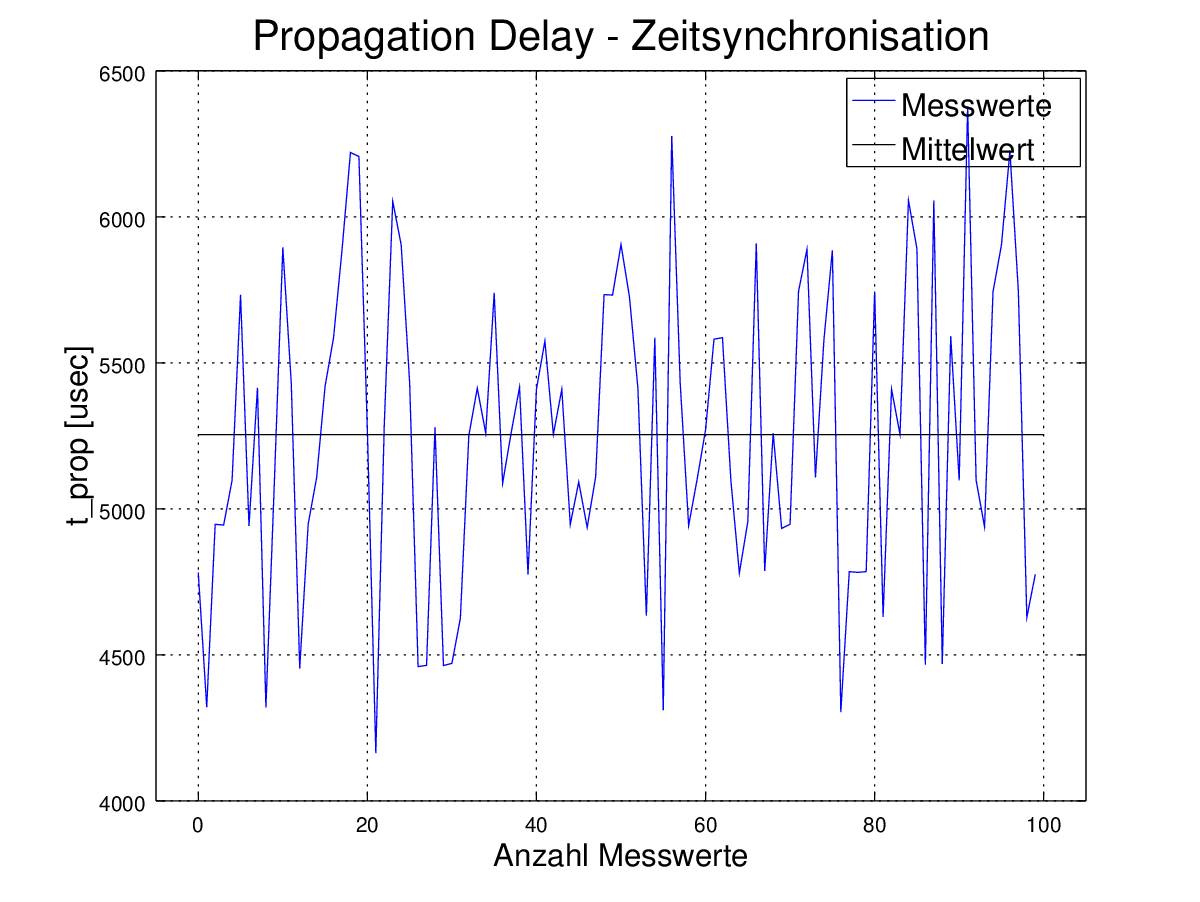
\includegraphics[width=1.2\textwidth]{images/t_prop_zeit_sync_figure.png}
        \caption{Messwerte von $t_{prop}$ bei hundert Messungen}
        \label{img:zeit_sync_t_prop_figure}
\end{figure}

Die obige Abbildung \ref{img:zeit_sync_t_prop_figure} zeigt die Laufzeitverzögerung bei \si{100} Messungen. Da die Messwerte sich im Millisekundenbereich bewegen, bedeutet dies für die Zeitsynchronisation falsche Ergebnisse. PTP verlangt für Zeitsynchronisation gleiche Laufzeitverzögerungen. Da diese im Millisekundenbereich schwanken, ist es zu erheblichen Abweichungen bei der Synchronisation gekommen. Neben der Laufzeitverzögerung spielt noch das Hinzufügen der Systemzeit in das Paket eine Rolle. Je später die Systemzeit in das UDP-Paket eingefügt wird, desto weniger Fehler gibt es bei der Zeitsynchronisation. Bei PTP muss die Systemzeit genau dem Aussenden entsprechen; deswegen ist die Systemzeit so spät wie möglich zum Paket hinzuzufügen. Passiert dies nicht, geht Genauigkeit verloren, weil das Zusammenbauen des UDP-Pakets Zeit kostet. Eine Vermutung für die Abweichungen bei der Laufzeitverzögerung ist, dass die Funktion $udp\_receive\_packet()$ durch Polling abgefragt wird. Somit gehen Pakete verloren und werden nur zu einem bestimmten Zeitpunkt entgegengenommen. RIOT bietet keine Interruptroutine für das Empfangen von Paketen an. Somit können Pakete verloren gehen, welches sich kritisch auf die Zeitsynchronisation auswirkt. Weiterhin ist eine kleine Abweichung von Master und Slave nicht zu verhindern. Da jeder Frequenzgeber schwingt, kommt nicht jeder Taktpegel exakt genau an. Der Jitter gibt an, um wieviele Nanosekunden der Frequenzgeber abweichen kann. Dieser ist beim Master und Slave minimal unterschiedlich.

\subsection{\funkempfaenger}
Um die Abweichung der Zeitsynchronisation aufzufangen, wird der \funkempfaenger \platz für das Startsignal einer Messung verwendet. Dafür muss allerdings der Empfänger ein eindeutiges Signal erhalten. Dies ist ein \si{LOW}-Signal. Da eine solche Abweichung für eine zentimetergenaue Positionsbestimmung nicht vertretbar ist, wird für den Start der Messung ein \funkempfaenger \platz verwendet. Für den Testaufbau wurde der Empfänger an das Oszilloskop angeschlossen. Der \si{DATA}-Eingang des Senders wurde mit dem \board \platz verbunden. Das Board produziert eine \SI{1}{\hertz} Frequenz auf dem verbunden Pin. Das Oszilloskop sollte nun diese Frequenz wiederspiegeln. Das Messergebnis ist in Abbildung \ref{img:ausgang_sender_pin} dargestellt. Es ist zu erkennen, dass das Mikrofon ein Rauschen erkennt. Dies belegen die vielen kurzen \si{LOW}-Pegel. Als vom Sender ein \si{LOW}-Pegel übertragen wurde, konnte nicht eindeutig bestimmt werden, ob das Signal angekommen war oder durch das Rauschen unterging. Die Pegelwechsel A-E belegen, dass sich kein Pegelwechsel am Ausgang eindeutig vom Rauschen abhebt. Somit kann diese Variante nicht als Startsignal verwendet werden. Der Funkempfänger scheidet damit aus.

\begin{figure}[H]
        \centering
        \hspace*{-1.7cm}
        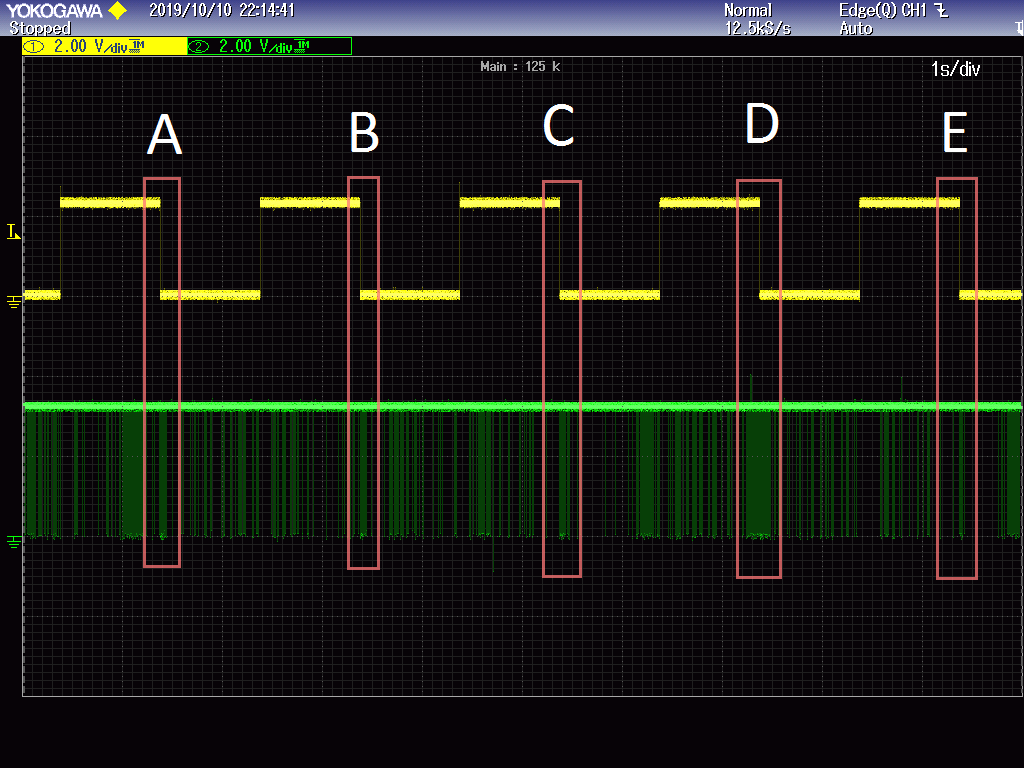
\includegraphics[width=1.2\textwidth]{images/schmitt_trigger_billig_sender_bearbeitet.png}
        \caption{\si{DATA}-Pin des \funkempfaenger \platz Empfänger}    
        \label{img:ausgang_sender_pin}
\end{figure}

\subsection{Software}
Für die Positionsbestimmung verhält sich die Software nach dem Programmablaufplan - siehe Abbildung \ref{img:PAP}. Zuerst wird der Zeitunterschied ausgeglichen, der zwischen dem Master und dem Slave besteht. Dafür wird das bereits beschriebene PTP Protokoll verwendet. Erst nachdem die Zeitsynchronisation erfolgreich ist, werden Messungen vorgenommen. Dabei spricht der Master einzeln die Slaves an. Der Master gibt zu einem bestimmten Zeitpunkt vor, wann der entsprechende Slave den Lautsprecher für \SI{40000}{\mu\s} einschaltet. Über das Mikrofon beim Master wird der Ton empfangen und sofort die Systemzeit bestimmt. Über die Differenz vom Aussenden und Empfangen kann die Distanz berechnet werden.
\begin{figure}[H]
        \centering
        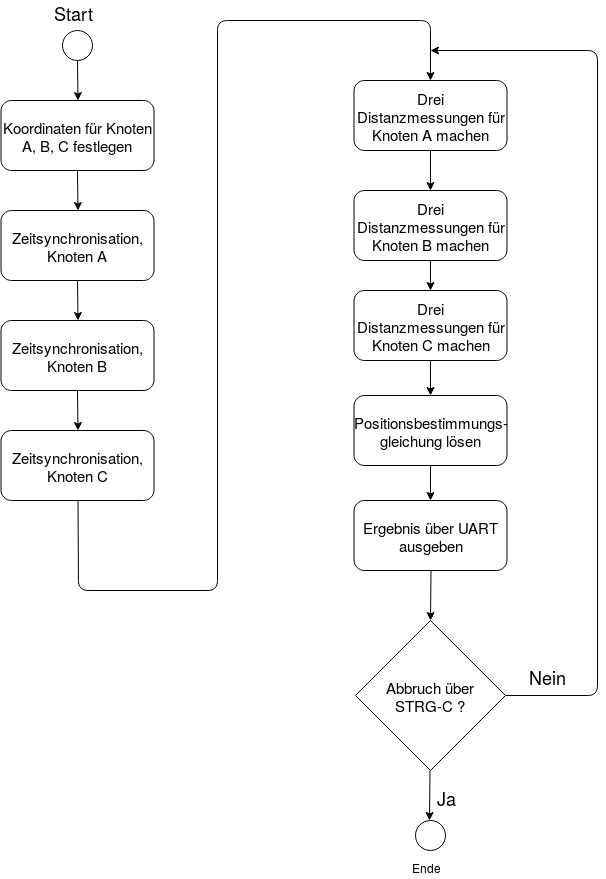
\includegraphics[width=0.8\textwidth]{images/PAP.png}
        \caption{Programmablaufplan der Software}
        \label{img:PAP}
\end{figure}

Dieses Vorgehen wird für alle drei Slaves wiederholt. Zusammen mit den Koordinaten der Slaves ergeben sich auf einer Ebene drei Kreise, die sich schneiden. Der Schnittpunkt der Kreise ist foglich die Position des Masters. Dabei ist zu beachten, dass der Master sich während der drei Messungen nicht bewegen darf - sonst werden die Ergebnisse verfälscht. Mit den drei Distanzen wird die Position bestimmt. Die Funktion für die Positionsbestimmung wurde von Github (pepebecker/circle-intersection) entnommen \cite{src_GITHUB_CODE}. Wird die Software nicht abgebrochen, wiederholt sich die Messung für alle Slaves. Somit kann sich der Master auf der Ebene bewegen und bekommt seine Postion angezeigt. Es muss beachtet werden, dass durch den Jitter des Frequenzgebers die Systemzeit der Slaves mit der Zeit divergiert, d.h, wartet man entsprechend lange, ist die Systemzeit der Slaves nicht mehr übereinstimmend mit dem Master. Deswegen muss regelmäßig eine Zeitsynchronisation erfolgen. Da diese Arbeit unter Laborbedinungen durchgeführt wird, gibt es nur eine Zeitsynchronisation.


\newpage
\section{Unit Test}

Unittests werden benötigt um die Software auf ihre Korrektheit zu überprüfen. Für diese Software werden nur Teilbereiche getestet, da viele Funktionen von der Peripherie abhängig ist.

\subsection{Quadratische Gleichung}
Für die Positionsbestimmung muss eine quadratisch Gleichung gelöst werden. Die Parameter für diese Funktion sind \si{p} und \si{q}. Diese entsprechen der Variablen aus der folgenden Gleichung:

\begin{equation}
\label{eq:unit_test_pq_formel}
x^{2} + p \cdot x + q = 0
\end{equation}

Es folgt eine Tabelle mit den Eingaben der Funktion und den dazugehörigen Ausgaben/ Rückgabewerten. 

\begin{table}[H]
\centering
\caption{Eingaben und Ausgaben der pq-Funktion}
\label{table:pq_funktion}
\begin{tabular}{|c|c|c|c|}
\hline
\multicolumn{2}{|c|}{\textbf{Eingaben}} & \multicolumn{2}{c|}{\textbf{Ergebnis}} \\ \hline
\textbf{p}         & \textbf{q}         & \textbf{x1}        & \textbf{x2}       \\ \hline
3                  & 2                  & -1                 & -2                \\ \hline
4                  & 1                  & -0,26                   & -3,73                  \\ \hline
-3                 & -9                 & 4,85                   & -1,85                  \\ \hline
\end{tabular}
\end{table}

Aus der Tabelle \ref{table:pq_funktion} wird deutlich das die Funktion korrekte Rückgabewerte liefert. Bei einer fehlerhaften Eingabe gibt die Funktion ein \si{NaN} (Not a Number) zurück.


\subsection{Abstand zweier Punkte}
Bei der Positionsbestimmung kann es dazu kommen, dass die drei Kreise sich nicht treffen. Dann haben wir zwei Punkte Bereiche indem der Knoten sich befindet. Um den korrekten Bereich zu bestimmen, wird die Funktion $determine\_point\_radius()$ benötigt. Liefert diese Funktion ein falsches Ergebnis führt das dazu das die Positionsbestimmung nicht mehr korrekt ist. Der korrekte Bereich kann bestimmt werden indem von zwei Punkten die Distanz zu einem Kreismittelpunkt bestimmt wird. Ein Punkt liegt innerhalb des Radius und der andere außerhalb. Der Punkt mit der geringsten Distanz ist der korrekte Punkt und makiert einen Eckpunkt des Bereichs indem sich der Knoten befindet. Die folgende Abbildung verdeutlicht das Problem.

\begin{figure}[H]
	\hspace*{-3.5cm}
    \subfigure[Positionsbestimmung ohne Schwankung]
    {
    	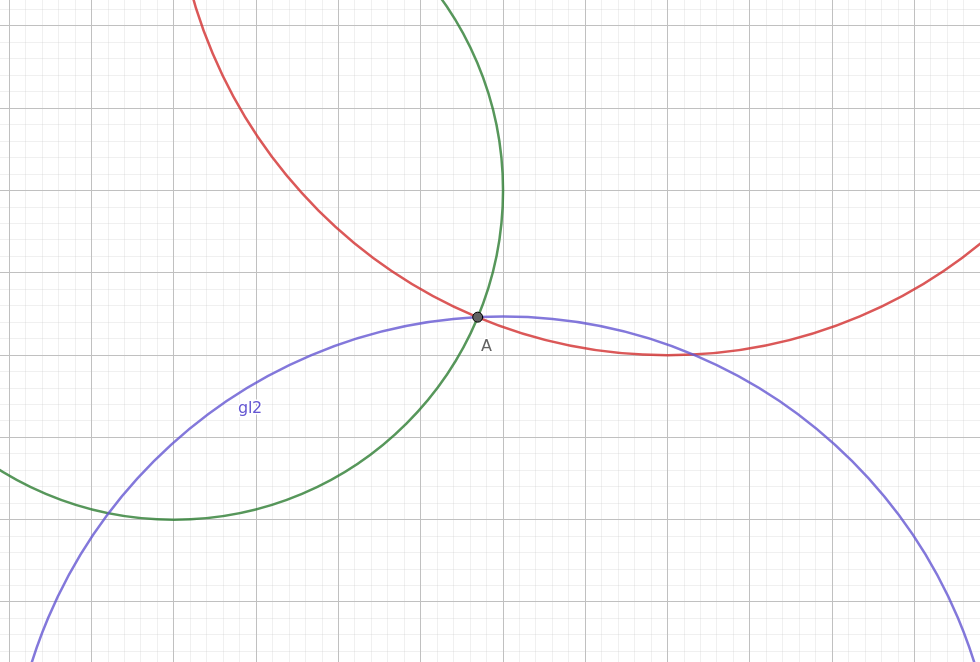
\includegraphics[width=0.7\textwidth]{images/picture_unit_test_calc_position_1.png}
    }
    \subfigure[Positionsbestimmung mit Schwankung]
    {
    	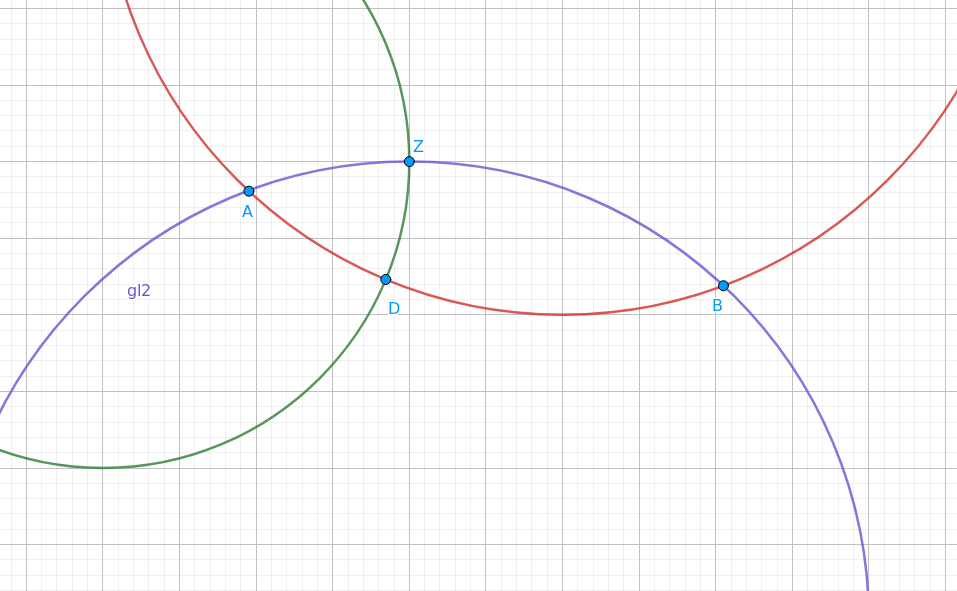
\includegraphics[width=0.7\textwidth]{images/picture_unit_test_calc_position_2.png}
    }
	\caption{Zwei Möglichkeiten der Positiosbestimmung}
	\label{img:figure_abstand_zweier_punkte}
\end{figure}

Aus der Abbildung \ref{img:figure_abstand_zweier_punkte} wird erkennbar, dass es durch die Schwankung zwei Bereiche geben kann. Ein Bereich durch die Eckpunkte \si{A}, \si{Z} und \si{D} und ein zweiter durch \si{B}, \si{Z} und \si{D} abgesteckt. Um nun zu bestimmen ob Punkt \si{A} oder \si{B} den Bereich ausgegangen von dem grünen Kreis kennzeichnet wird der Abstand zum Kreismittelpunkt vom grünen Kreis berechnet. Die Funktion wird mit den folgenden zwei Punkten und der Kreisgleichung getestet.

\begin{equation*}
\label{eq:unit_test_abstand_zweier_punkte}
\begin{split}
P_{A}: \; (3,9528 \;|\; 2,8069)\\
P_{B}: \; (7,0504 \;|\; 2,1899)\\
(x - 3)^{2} + (y - 3)^{2} = 2^{2}
\end{split}
\end{equation*}

Punkt \si{A} ist der korrekte Punkt weil sein Abstand zum Kreismittelpunkt kleiner ist als von Punkt \si{B} ($0.9721 < 4.1306$) und daher sollte er von der Funktion zurückgegeben werden. Die Funktion funktioniert wie erwartet fehlerfrei.

\subsection{Positionsbestimmung}
Zur Bestimmung der Position braucht die Funktion drei Parameter. Diese sind die drei Kreise die sich im einem Schnittpunkt schneiden oder ein Bereich aufspannen. Für den Fall das alle drei Kreise einen gemeinsamen Schnittpunkt haben gibt die Funktion dreimal die X/Y-Koordinaten zurück. Bei einem Bereich werden die X/Y-Koordinaten der Eckpunkte zurückgegeben. Die Funktion wird mit den folgenden Kreisgleichungen getestet.  Zuerst ein Test wobei es ein gemeinsamen Schnittpunkt gibt.

\begin{equation*}
\label{eq:unit_test_positionsbestimmung}
\begin{split}
(x - 3)^{2} + (y - 3)^{2} = 2^{2} \\
(x - 6)^{2} + (y - 2)^{2} = 2^{2} \\
(x - 4)^{2} + (y - 1,8693)^{2} = 2^{2}
\end{split}
\end{equation*}
Der Schnittpunkt der drei Kreise ist $( 4,8872 \;|\; 3,6618)$. Dies gibt auch die Funktion zurück. Als nächtes wird der Rückgabewert bei keinem gemeinsamen Schittpunkt untersucht.

\begin{equation*}
\label{eq:unit_test_positionsbestimmung}
\begin{split}
(x - 3)^{2} + (y - 3)^{2} = 2^{2} \\
(x - 6)^{2} + (y - 2)^{2} = 2^{2} \\
(x - 4)^{2} + (y - 5)^{2} = 2^{2}
\end{split}
\end{equation*}

Die obigen drei Kreise haben keinen gemeinsamen Schittpunkt. Die Funktion gibt die folgenden Koordinaten der Eckpunkte zurück.

\begin{equation*}
\label{eq:unit_test_positionsbestimmung_2}
\begin{split}
P_{A}: \; (4,8872 \;|\; 3,6618)\\
P_{B}: \; (4,9832 \;|\; 3,2583)\\
P_{C}: \; (4,2794 \;|\; 3,0196)
\end{split}
\end{equation*}

In beiden Fällen ist der Rückgabewert der Funktion korrekt. Somit funktioniert die Funktion wie erwartet.







\newpage
\section{Auswertung}

Nachdem die Implementierung abgeschlossen ist, widmen wir uns in diesem Kaptiel der Auswertung der Daten.

\subsection{Hardware}
Die aufgetretenen Abweichungen entstanden meistens, wenn die Peripherie Daten generiert hat bzw. angesprochen wurde. Da viele dieser Abweichungen konstant sind, kann ein Offset für ein korrektes Ergebnis mit in das Ergebnis einfließen. Allerdings sind einige Abweichungen nicht erklärbar, was die Bestimmung eines Offset erschwert. Weiterhin zeigt sich, dass die verwendete Hardware nicht optimal auf dieses Problem abgestimmt ist. Dazu zählt der Tongeber und das  \microphone . RIOT sieht sich zwar als Echtzeitbetriebssystem, allerdings sind zu viele Schichten zwischen dem laufenden Programm und der Hardware, denn ein Systemaufruf für die Abfrage der Systemzeit darf nicht \SI{7,21}{\mu s} dauern. Dies verfälscht die Systemzeit die eigentlich \si{\mu}-Sekunden genau sein soll. Des weiteren zeigt sich, desto weniger Komponenten (Peripherie) verwendet wird, desto einfacher ist die Fehlersuche. Eine Laufzeitmessung könnte z.B. im Funkchip enthalten sein. Somit spart man sich aufwendige Peripherie. 

\subsection{Messergebnis}
Die Messergebnisse zeigen, dass eine Positionsbestimmung auf diese Weise nicht genau genug ist. Die Abweichung, die das Messergebnis hauptsätlich verfälscht, liegt beim Tongeber und dem Mikrofon. Weil kein Muster bei der Abweichung erkennbar ist, kann kein Offset bestimmt werden. Weiterhin liefert das Oszilloskop die gleichen Abweichungen für alle verwendeteten Mikrofone, sodass die Verwendung eines fehlerbehafteten Bausteins ausgeschlossen werden kann. 

\subsection{Software}

Die Software kann eine Positionsbestimmung durchführen, dabei ist sie allerdings auf korrekte Distanzmesswerte angewiesen. Da diese fehlen, kann die Software nur durch Unit-Tests validiert werden.






\newpage
\section{Probleme}
Dieser Abschnitt wendet sich den Problemen zu, die erst bei der Durchführung dieser Arbeit aufgetreten sind und vorher nicht abzuschätzen waren.

\subsection{Kommunikation Master -- Slave}
Der Forschungsansatz der drahtlosen Kommunikation im Rahmen dieser Bachelorarbeit bestand darin, dass Steuerkommandos und Daten immer getrennt gesendet und immer auf 32-Bit aligned werden. Das hat zur Folge, dass Daten immer vom vorherigen Steuercode abhängig sind. Kommt der Steuercode nicht beim Empfänger an, können nachfolgende Daten dem nicht zugeordnet bzw. korrekt interpretiert werden. Die Kommunikation war serialisiert -- die nächsten Daten konnten nur interpretiert werden, wenn die vorherigen Daten fehlerfrei ankamen. Da es häufig zu nicht erklärbaren Verbindungsabbrüchen während der Kommunikation kam, wurde die serialisierte Kommunikationsvariante durch Structs abgelöst. Dabei enthalten die Structs den Steuercode und die dazugehörigen Daten. Somit liegen Steuercodes und Daten zusammen. Sollten nun Daten verloren gehen, können durch den dazugehörigen Steuercode nachfolgende Daten weiterhin interpretiert werden. Die Kombination von Daten und Steuercodes ermöglicht eine variable Kommunikation. Dadurch ist man nicht mehr abhängig von den vorherigen Daten.

\subsection{Genauigkeit -- Zeitsynchronisation}
Im Rahmen der Zeitsynchronisation kam es immer wieder zu dem Problem, dass die Genauigkeit bei mehrfachen Wiederholungen nicht besser wurde. Dadurch, dass sich die Zeitsynchronisation nicht im \si{\mu}-Sekundenbereich auflöste, konnten auch nur Messungen mit größeren Abweichungen erfolgen. Die Abweichung kam insbesondere durch die Aufrufe $getSystemTime()$ und $udp\_send\_packet()$ zustande. Die Systemzeit wurde vor dem Aussenden vom Programm selbst in das Datenpaket eingefügt und nicht von der Firmware des Funksenders. Weiterhin baute die Funktion $udp\_send\_packet()$ zuerst das UDP-Paket zusammen, welches wiederum Zeit kostete, bis es gesendet werden konnte.

\subsection{Genauigkeit -- Messungen}
Theoretisch ist nach einer Zeitsynchronisation bekannt, um wie viel Zeit der Master dem Slave hinterher hängt, bzw. voraus ist. Bei den praktischen Distanzmessungen mit dem Slave kam es dabei immer wieder zu großen Distanzschwankungen. Diese haben vermutlich drei Ursachen: eine nicht im \si{\mu}-Sekundenbereich auflösende Zeitsynchronisation, eine Verzögerung der Messinstrumente sowie eine Ablenkung des Schalls vom Aussenden bis zum Empfangen des Mikrofons.
\newpage

\section{Ausblick}
Die Software kann man in verschiedenen Module einteilen. Dadurch ist es möglich, die Software zu erweitern ohne die anderen Module zu verändern. Folgend werden Verbesserungsvorschläge für die einzelnen Module vorgestellt.

\paragraph{Kommunikation}\mbox{}\\
Für die Kommunikation zwischen Master und Slave, könnte anstatt des UDP-Protokoll das TCP-Protokoll verwendet werden. Dadurch wird eine fehlerbehaftete Kommunikation verbessert, weil TCP mit ACKs arbeitet und zuerst ein Verbindungsaufbau erfolt. Darüber hinaus könnte die Identifikation der Knoten im Netzwerk mit einer IP-Adresse erfolgen, anstatt auf Portnummern wie es aktuell ist.

\paragraph{Zeitsynchronisation}\mbox{}\\
Damit eine Uhrensynchronisation im Nanosekundenbereich erreicht wird, muss die aktuelle Uhrzeit kurz vor dem Aussenden in das Datenpaket eingefügt werden. Dies sollte unabhängig vom System geschehen. Dafür muss die Systemzeit von der Firmware des Funkmoduls verwaltet werden. Wird die Systemzeit allerdings vom Betriebssystem verwaltet, gibt es immer eine Verzögerung von dem Funktionsaufruf $getSystemTime()$ und dem Aussenden des Pakets. Genau um diese Verzögerungszeit zu elemenieren, sollte bei jedem Aussenden des Paketes die aktuelle Systemzeit angehängt werden.

\paragraph{Übertragungsmedium}\mbox{}\\
Anstatt von Schall, können auch Radiosignale verwendet werden. Diese haben den Vorteil das das menschliche Gehör diese Frequenzen nicht wahrnimmt. Des weiteren breiten sich Radiosignale mit Lichtgeschwindigkeit aus. Zusammen mit einer Frequenzmodulationen können mehrere Accesspoints gleichzeitig abgefragt werden. Dies ermöglicht eine schnellere Positionsbestimmung. Radiosignale haben den Nachteil, dass eine Dämpfung bei Wänden stattfindet. Weitherhin muss bedacht werden, dass es zu Reflexionen, Streuung und Absorbation kommen kann \cite{src_RADIOSIGNALE}.

\paragraph{Messung}\mbox{}\\
Für die Positionsbestimmung müssen drei Gleichungen gelöst. Da MCUs nicht immer über eine FPU verfügen, kann eine MCU mit FPU verwendet werden. Oder ein Raspberry-Pi, denn dieser ermöglicht die gemessenen Daten mit Octave oder Matlab weiter zu verarbeiten. Das hat den Vorteil, dass die Berechnung durch die FPU beschleunigt wird. Darüber hinaus ermöglicht Octave, Statistiken oder graphische Aufbereitung der Daten.

\paragraph{Hardware}\mbox{}\\
Aktuell ist der Lautsprecher und das Mikrofon über ein Steckbrett mit dem \board \platz verbunden. Es könnte eine Leiterplatte angefertigt werden, die auf das \board \platz aufgesteckt wird. Das würde eventuelle Fehler beim Steckbrett vermeiden.  

\paragraph{Signalanalyse}\mbox{}\\
Um genauer herrauszufinden, wann das Signal beim Mikrofon ankommt, kann eine Signalanalsye durchgeführt werden. Es könnte immer die Zeit gestoppt werden, wenn die Amplitude erste Halbwelle der Sinusschwinkung erkannt wird, oder eine Periode vorbei ist. Dadurch ist es dann möglich, einen definierten Zeitpunkt zu bestimmen, wann das Lautsprechersignal das Rauschen am \si{AUDIO}-Ausgang überlagert. Der Lautsprecher muss dafür aber ein Signal zurückgeben, wann die erste Halbwelle erreicht wurde.

\paragraph{Betriebssystem}\mbox{}\\
Anstatt das Betriebssystem RIOT zu verwenden, kann auch ein eigenes Betriebssystem geschrieben und verwendet werden. Dies ermöglicht eine bessere Programmanalyse über das laufende Programm. Darüber hinaus können eventuelle Softwareroutinen, die nicht unbedingt essentiell sind, abgeschaltet werden, bzw. gar nicht erst implementiert werden. Weiterhin könnte RIOT OS angepasst/ erweitert werden.






%Ausblick
\newpage
\section{Zusammenfassung}


Muss noch geschrieben werden ....

\newpage
\addcontentsline{toc}{section}{Eidesstattliche Erklärung}
%\section*{Eidesstattliche Erklärung}
\section*{Eidesstattliche Erklärung\markboth{EIDESSTATTLICHE ERKLÄRUNG}{EIDESSTATTLICHE ERKLÄRUNG}}

Ich erkläre hiermit an Eides Statt, dass ich die vorliegende Arbeit selbstständig und ohne Benutzung anderer als der angegebenen Hilfsmittel angefertigt habe; die aus fremden Quellen direkt oder indirekt übernommenen Gedanken sind als solche kenntlich gemacht. Die Arbeit wurde bisher in gleicher oder ähnlicher Form keiner anderen Prüfungskommission vorgelegt und auch nicht veröffentlicht.
\\
\\
Berlin, 17.12.2019
\\
\\
\\
\underline{\hspace{5cm}}
\\
Oliver Koepp


\newpage

sdfbsbf\cite{src_tdoa}


\addcontentsline{toc}{section}{Literaturverzeichnis}
\section*{Literaturverzeichnis\markboth{Literaturverzeichnis}{LITERATURVERZEICHNIS}}

\begin{thebibliography}{}

%%%%%%%%%%%%%%%%%%%%%%%%%%%%%%%%%%%%%%%%
%Einleitung
%%%%%%%%%%%%%%%%%%%%%%%%%%%%%%%%%%%%%%%%
\bibitem{src_CE_CAR}
	\textit{CE-Car} - URL \url{https://ce-master.htw-berlin.de/} - abgerufen am 12.09.2019


	

%Indoor/Outdoor Systeme
\bibitem{src_INDOOR_OUTDOOR}
	\textit{In- und Outdoor Positionierungssysteme} - URL \url{https://pi4.informatik.uni-mannheim.de/pi4.data/content/courses/2005-ws/seminar/Vortrag_Positionierung-Uebersicht_Indoor_und_Outdoor_Positionierungssysteme.pdf} - abgerufen am 7.7.2019	

%%%%%%%%%%%%%%%%%%%%%%%%%%%%%%%%%%%%%%%%
%Grundlagen
%%%%%%%%%%%%%%%%%%%%%%%%%%%%%%%%%%%%%%%%


\bibitem{src_SAMR}
	\textit{Atmel SAM R21} - URL \url{https://riot-os.org/api/group__boards__samr21-xpro.html} - abgerufen am 02.07.2019	


\bibitem{src_HC_SR04}
	\textit{Ultraschall Sensor HC-SR04 und kompatible Ultraschall-Module} 2016 - URL \url{https://www.mikrocontroller-elektronik.de/ultraschallsensor-hc-sr04/} - abgerufen am 03.09.2019	


\bibitem{src_SOUND_DETECTOR}
	\textit{Sound Detector Hookup Guide} - URL \url{https://learn.sparkfun.com/tutorials/sound-detector-hookup-guide} - abgerufen am 09.09.2019	

\bibitem{src_433_FUNKSENDER}
	\textit{433 Mhz Funk Transmitter-Receiver} - URL \url{https://draeger-it.blog/arduino-tutorial-433mhz-sender-empfaenger/} - abgerufen am 18.10.2019	

\bibitem{src_LAUTSPRECHER}
	\textit{Goliton 5X Alarm 95dB Hohe Dezibel 6-24V 12V elektronischer Summer kontinuierlicher Piep Arduino MFC-27} - URL \url{https://www.amazon.de/Goliton-Dezibel-elektronischer-kontinuierlicher-Arduino/dp/B01MT5V0FM/ref=sr_1_1?__mk_de_DE=\%C3\%85M\%C3\%85\%C5\%BD\%C3\%95\%C3\%91&keywords=Goliton+5X+Alarm+95dB+Hohe+Dezibel+6-24V&qid=1572779993&sr=8-1} - abgerufen am 01.08.2019	

\bibitem{src_RIOT}
	\textit{RIOT-The friendly Operating System for the Internet of Things} - URL \url{https://riot-os.org/} 2013 - abgerufen am 30.07.2019	


\bibitem{src_TDOA}
	\textit{TIME DIFFERENCE OF ARRIVAL} - URL \url{https://www.sewio.net/uwb-technology/time-difference-of-arrival/} - abgerufen am 04.07.2019	


\bibitem{src_UDP}
	\textit{UDP - User Datagram Protocol} - URL \url{https://www.elektronik-kompendium.de/sites/net/0812281.htm} - abgerufen am 25.08.2019	

\bibitem{src_SOCKET}
	\textit{Introduction to RAW-sockets} - URL \url{https://tuprints.ulb.tu-darmstadt.de/6243/1/TR-18.pdf} - abgerufen am 14.08.2019	

\bibitem{src_INDOOR_OUTDOOR_SYSTEME}
	\textit{In- und Outdoor
Positionierungssysteme} - URL \url{https://pi4.informatik.uni-mannheim.de/pi4.data/content/courses/2005-ws/seminar/Vortrag_Positionierung-Uebersicht_Indoor_und_Outdoor_Positionierungssysteme.pdf} 

\bibitem{src_PTP}
	\textit{A Sub-Microsecond Clock Synchronization Protocol for Wireless Industrial Monitoring and Control Networks} 2017 - URL \url{https://www.ibr.cs.tu-bs.de/oa/vonzengen_ICIT2017.pdf} - abgerufen am 26.08.2019

 
\bibitem{src_MATH_TDOA}
	\textit{Finding Location with Time of Arrival and Time Difference of Arrival Techniques} - URL \url{https://sites.tufts.edu/eeseniordesignhandbook/files/2017/05/FireBrick_OKeefe_F1.pdf} 2017 - abgerufen am 11.07.2019	
	
%%%%%%%%%%%%%%%%%%%%%%%%%%%%%%%%%%%%%%%%
%Implementierung
%%%%%%%%%%%%%%%%%%%%%%%%%%%%%%%%%%%%%%%%


\bibitem{src_GITHUB_CODE}
	\textit{Software zur Positionsbestimmung} 2019 - URL \url{https://github.com/pepebecker/circle-intersection} - abgerufen am 28.10.2019	
	
	
%%%%%%%%%%%%%%%%%%%%%%%%%%%%%%%%%%%%%%%%
%Ausblick
%%%%%%%%%%%%%%%%%%%%%%%%%%%%%%%%%%%%%%%%	
\bibitem{src_RADIOSIGNALE}
	\textit{Funktechnik (Grundlagen)} 2019 - URL \url{https://www.elektronik-kompendium.de/sites/kom/0810301.htm} - abgerufen am 06.11.2019	
	
%%%%%%%%%%%%%%%%%%%%%%%%%%%%%%%%%%%%%%%%
%Ausblick
%%%%%%%%%%%%%%%%%%%%%%%%%%%%%%%%%%%%%%%%		
\bibitem{src_GITHUB_CODE_BA}
\textit{Bachelorarbeit} 2019 - URL \url{https://github.com/git-oliver/Bachelorarbeit} - abgerufen am 09.11.2019	
	
	
	
	
	
	
	
	
\end{thebibliography}

\newpage
%\appendix
\section{Anhang}

\subsection{Mathematische Herleitung}
\label{sec:abcdef}
Diese Arbeit zeigt die Herleitung, nur für einen Punkt aus der Abbildung \ref{img:schwankungen}, denn die Herleitungen der anderen beiden Punkte unterscheiden sich nur in den Variablen $x_{A}$, $y_{A}$ und $r_{A}$.
Zuerst wird eine Geradengleichung bestimmt, die durch die beiden Schnittpunkte von Kreis $A$ und $B$ gehen.

%\begin{equation}\label{eq:gerade_bestimmen}
%\begin{split}
%\RM{1} \quad (x-x_{A})^{2}+(y-y_{A})^{2} &= r_{A}^{2} \\
%\RM{2} \quad (x-x_{B})^{2}+(y-y_{B})^{2} &= r_{B}^{2} \\
%\cline{1-2}
%\RM{1} - \RM{2} \quad
%x \cdot (2 \cdot x_{B}-2 \cdot x_{A}) + y \cdot (2 \cdot y_{B}-2 \cdot y_{A}) + x_{A}^{2} - x_{B}^{2} + y_{A}^{2} - y_{B}^{2} &= r_{A}^{2} - r_{B}^{2} \\
%\RM{1} - \RM{2} \quad
%x \cdot (2 \cdot x_{B} - 2 \cdot x_{A}) + y \cdot (2 \cdot y_{B} - 2 \cdot y_{A}) &= r_{A}^{2} - r_{B}^{2} - x_{A}^{2} + x_{B}^{2} - y_{A}^{2} + y_{B}^{2} \\
%\RM{1} - \RM{2} \quad y = \frac{ x \cdot (2 \cdot x_{A} - 2 \cdot x_{B}) + r_{A}^{2} - r_{B}^{2} - x_{A}^{2} + x_{B}^{2} - y_{A}^{2} + y_{B}^{2} }{2 \cdot (y_{B} - y_{A})}
%\end{split}
%\end{equation}

\noindent
$
\RM{1} \hspace{5.7cm} (x-x_{A})^{2}+(y-y_{A})^{2} = r_{A}^{2} \\
\RM{2} \hspace{5.5cm} (x-x_{B})^{2}+(y-y_{B})^{2} = r_{B}^{2} \\
\RM{1}-\RM{2} \hspace{0.3cm} x \cdot (2 \cdot x_{B}-2 \cdot x_{A}) + y \cdot (2 \cdot y_{B}-2 \cdot y_{A}) + x_{A}^{2} - x_{B}^{2} + y_{A}^{2} - y_{B}^{2} = r_{A}^{2} - r_{B}^{2}
$
\begin{equation}\label{eq:geradengleichung}
\hspace{1cm} y = \frac{ x \cdot (2 \cdot x_{A} - 2 \cdot x_{B}) + r_{A}^{2} - r_{B}^{2} - x_{A}^{2} + x_{B}^{2} - y_{A}^{2} + y_{B}^{2} }{2 \cdot (y_{B} - y_{A})}
\end{equation}

Um nun die X-Koordinaten zu bekommen, setzen wir die Gleichung \ref{eq:geradengleichung} in Gleichung $\RM{1}$ ein und lösen nach $x$ auf.

\begin{equation}\label{eq:x_aufloesen}
\begin{split}
P = r_{A}^{2} - r_{B}^{2} - x_{A}^{2} + x_{B}^{2} - y_{A}^{2} + y_{B}^{2}
\\
(x-x_{A})^{2}+(y-y_{A})^{2}&=r_{A}^{2}\\
(x-x_{A})^{2} + (\frac{ x \cdot (2 \cdot x_{A} - 2 \cdot x_{B}) + P}{2 \cdot (y_{B} - y_{A})} - y_{A})^{2}&=r_{A}^{2}
\\
x^{2}(1+(\frac{x_{B}-x_{A}}{y_{B}-y_{A}})^{2}) + x (\frac{-P \cdot (x_{B} - x_{A})}{(y_{B} - y_{A})^{2}} + \frac{2 \cdot y_{A} \cdot (x_{B}-x_{A})}{y_{B} - y_{A}} - 2 \cdot x_{A}) \\
= r_{A}^{2} - y_{A}^{2} + \frac{y_{A} \cdot P}{y_{B}-y_{A}} - \frac{P^{2}}{4 \cdot (y_{B}-y_{A})^{2}} - x_{A}^{2}
\\
(1+(\frac{x_{B}-x_{A}}{y_{B}-y_{A}})^{2}) &= R
\\
(\frac{-P \cdot (x_{B} - x_{A})}{(y_{B} - y_{A})^{2}} + \frac{2 \cdot y_{A} \cdot (x_{B}-x_{A})}{y_{B} - y_{A}} &= S
\\
r_{A}^{2} - y_{A}^{2} + \frac{y_{A} \cdot P}{y_{B}-y_{A}} - \frac{P^{2}}{4 \cdot (y_{B}-y_{A})^{2}} - x_{A}^{2} &= T
\\
\\
x^{2} + x \cdot \frac{S - 2 \cdot x_{A}}{R} - \frac{T}{R} = 0
\end{split}
\end{equation}
Zum lösen einer quadratischen Gleichung wird die pq-Formel verwendet.
\begin{equation}\label{eq:x_aufloesen_pq_formel}
\begin{split}
p &= \frac{S - 2 \cdot x_{A}}{R}
\\
q &= \frac{T}{R}
\\
\\
x_{1,2} &= -\frac{p}{2} \pm \sqrt{(\frac{p}{2})^{2} -q}
\\
x_{1} &= -\frac{p}{2} + \sqrt{(\frac{p}{2})^{2} -q}
\\
x_{2} &= -\frac{p}{2} - \sqrt{(\frac{p}{2})^{2} -q}
\end{split}
\end{equation}

Nachdem die X-Koordinaten ermittelt worden sind, muss noch die Y-Koordinate für $x_{1}$ und $x_{2}$ bestimmt werden. Dafür werden die X-Koordinaten in die Geradengleichung \ref{eq:geradengleichung} eingesetzt.
\begin{equation}\label{eq:y_errechnen}
\begin{split}
\RM{1} \hspace{5.7cm} (x-x_{A})^{2}+(y-y_{A})^{2} = r_{A}^{2} \\
\hspace{1cm} y_{1} = \frac{ x_{1} \cdot (2 \cdot x_{A} - 2 \cdot x_{B}) + r_{A}^{2} - r_{B}^{2} - x_{A}^{2} + x_{B}^{2} - y_{A}^{2} + y_{B}^{2} }{2 \cdot (y_{B} - y_{A})}
\\
\hspace{1cm} y_{2} = \frac{ x_{2} \cdot (2 \cdot x_{A} - 2 \cdot x_{B}) + r_{A}^{2} - r_{B}^{2} - x_{A}^{2} + x_{B}^{2} - y_{A}^{2} + y_{B}^{2} }{2 \cdot (y_{B} - y_{A})}
\end{split}
\end{equation}

Die Schnittpunkte von Kreis $A$ und $B$ sind:
\begin{equation}\label{eq:schnittpunkte}
\begin{split}
(x_{1} | y_{1})
\\
(x_{2} | y_{2})
\end{split}
\end{equation}

Da nur ein Schnittpunkt auch in Kreis $C$ liegt, muss dieser bestimmt werden, sonst erhalten wir nicht minimalste Fläche, die drei Kreise erzeugen. Um zu prüfen, welcher Schnittpunkt in Kreis $C$ liegt, wird der Abstand vom Mittelpunkt des Kreises $C$ zu den Schnittpunkten aus Gleichung \ref{eq:schnittpunkte} berechnet.

\begin{equation}\label{eq:schnittpunkt_der_im_kreis_liegt}
\begin{split}
d_{1} = \sqrt{(x_{C} - x_{1})^2 + (y_{C} - y_{1})^{2}}
\\
d_{2} = \sqrt{(x_{C} - x_{2})^2 + (y_{C} - y_{2})^{2}}
\end{split}
\end{equation}

Wenn $d_{1} < d_{2}$ ist, dann ist der gesuchte Punkt $(x_{1} | y_{1})$. Falls die Ungleichung $d_{1} > d_{2}$ wahr ist, dann heißt der gesuchte Punkt $(x_{2} | y_{2})$.
\\
Dieses mathematische Vorgehen wird für Kreis $A-C$ und $B-C$ wiederholt.

\newpage
\subsection{Steuercodes}
Die folgende Tabelle listet alle vorhandenen Steuercodes auf.

\begin{table}[H]
\label{table:steuercodes}
\caption{Alle Steuercodes}
\centering
\begin{tabular}{ccc}
\hline
\multicolumn{1}{|c|}{\textbf{Steurcode}} & \multicolumn{1}{c|}{\textbf{\textit{unsigned int} Wert}} & \multicolumn{1}{c|}{\textbf{Beschreibung}} \\ \hline
& & \\ \hline
\multicolumn{1}{|c|}{\si{CODE\_MESSUNG}} & \multicolumn{1}{c|}{\si{65}} & \multicolumn{1}{c|}{Messung durchführen} \\ \hline
\multicolumn{1}{|c|}{\si{CODE\_NOP}} & \multicolumn{1}{c|}{66} & \multicolumn{1}{c|}{ACK anfordern} \\ \hline
\multicolumn{1}{|c|}{\si{CODE\_ZEIT\_SYNC}} & \multicolumn{1}{c|}{\si{67}} & \multicolumn{1}{c|}{\si{SYNC-MSG} senden} \\ \hline
\multicolumn{1}{|c|}{\si{CODE\_ZEIT\_FOLLOW\_UP}} & \multicolumn{1}{c|}{\si{68}} & \multicolumn{1}{c|}{\si{FOLLOW\_UP-MSG} senden} \\ \hline
\multicolumn{1}{|c|}{\si{CODE\_ZEIT\_DELAY\_REQ}} & \multicolumn{1}{c|}{\si{69}} & \multicolumn{1}{c|}{\si{DELAY\_REQ-MSG} senden} \\ \hline
\multicolumn{1}{|c|}{\si{CODE\_ZEIT\_DELAY\_RESP}} & \multicolumn{1}{c|}{\si{70}} & \multicolumn{1}{c|}{\si{DELAY\_RESP-MSG} senden} \\ \hline
\multicolumn{1}{|c|}{\si{CODE\_READ\_T1\_T2\_T4}} & \multicolumn{1}{c|}{\si{71}} & \multicolumn{1}{c|}{Zurücksenden der Werte $t_{1}$, $t_{2}$, $t_{4}$} \\ \hline
\multicolumn{1}{|c|}{\si{CODE\_SERVER\_RESPONSE}} & \multicolumn{1}{c|}{\si{72}} & \multicolumn{1}{c|}{\si{ACK}} \\ \hline

\end{tabular}
\end{table}

\shorthandon{"}

\end{document}

